\RequirePackage{float}
\documentclass[pdflatex,sn-mathphys-num]{sn-jnl}
\usepackage{cmap}
\usepackage[T2A]{fontenc}
\usepackage[utf8]{inputenc}
\usepackage{type1ec}
\usepackage[english,russian]{babel}
\usepackage{amsmath,amssymb,amsfonts,amsthm}
\usepackage{graphicx,booktabs,tabularx,array}

\usepackage{etoolbox,placeins,needspace}
\usepackage{fvextra}
\newcommand{\MultiCallRole}{\mbox{MultiCall-Role}}
\newcommand{\E}{\mathbb{E}}
\newcommand{\I}{\mathbb{I}}
\newcommand{\len}[1]{\lvert#1\rvert_{\mathrm{tok}}}
\theoremstyle{definition}
\newtheorem{proposition}{Утверждение}
\newtheorem{definition}{Определение}
\newtheorem{assumption}{Предположение}
\renewcommand{\keywordname}{Ключевые слова}
\newenvironment{formulakey}{\par\addvspace{.35\baselineskip}\noindent\begin{minipage}{\linewidth}
\setlength{\abovedisplayskip}{4pt}\setlength{\belowdisplayskip}{4pt}}{\end{minipage}\par\addvspace{.3\baselineskip}}
\newenvironment{symbols}{\par\nopagebreak\smallskip\small\noindent\textit{где:}\par\nopagebreak
\begin{list}{}{\setlength{\leftmargin}{1.05em}\setlength{\rightmargin}{0pt}\setlength{\topsep}{2pt}\setlength{\itemsep}{1pt}\setlength{\parsep}{0pt}}}{\end{list}\smallskip}
\newcommand{\sym}[2]{\item \(\displaystyle #1\) --- #2.}

\makeatletter
\patchcmd{\@maketitle}{Corresponding author(s). E-mail(s):}{Для корреспонденции:}{}{}
% Compact front matter without reducing the abstract font.
\patchcmd{\@maketitle}{\vskip21pt}{\vskip0pt}{}{}
\patchcmd{\@maketitle}{\vskip20pt}{\vskip6pt}{}{}
\patchcmd{\@maketitle}{\vskip20pt}{\vskip12pt}{}{}
\patchcmd{\@maketitle}{\vskip24pt}{\vskip10pt}{}{}
\patchcmd{\@maketitle}{\vskip24pt}{\vskip10pt}{}{}
\patchcmd{\@maketitle}{\vskip36pt}{\vskip8pt}{}{}
\renewcommand\abstracthead{\@startsection{section}{1}{\z@}{-12pt}{3pt}{\abstractheadfont}}
\def\abstractfont{\reset@font\fontsize{9bp}{11bp}\selectfont\leftskip=12pt\rightskip=12pt\parfillskip=0pt plus 1fil}
\makeatother
\setlength{\emergencystretch}{2em}
\begin{document}
\selectlanguage{russian}
\raggedbottom
\allowdisplaybreaks[0]
\title[Токенный бюджет при генерации кода]{Сравнение способов вызова языковых моделей для оптимизации токенного бюджета при генерации кода в~задачах программной инженерии}
\author*[1]{\fnm{Даниил} \sur{Привезенцев}}\email{daprivezentsev@edu.hse.ru}
\affil*[1]{\orgname{Национальный исследовательский университет <<Высшая школа экономики>>}, \orgaddress{\city{Москва}, \country{Россия}}}
\abstract{Чтобы написать или исправить программу, большой языковой модели (LLM) передают запрос (описание того, что нужно сделать) и~контекст (исходный код, документацию и~другие необходимые сведения). При нескольких вызовах контекст может передаваться повторно, увеличивая расход входных токенов.

В~статье сравниваются способы вызова одной и~той же LLM по расходу токенов, расчётной стоимости и~доле программ, успешно прошедших тесты. При \emph{интроспективном вызове} модели одним запросом поручают спланировать решение, написать и~проверить код. При \emph{последовательных вызовах} эти действия распределяют между тремя запросами. Каждый получает исходную задачу и~ответы предыдущих этапов, если они есть.

Пять экспериментальных серий выполнены на BigCodeBench, наборе задач на написание функций Python с~автоматическими тестами. В~серии на 1\,000 задачах программной инженерии завершён 14\,961 прогон LLM GPT-5.6 Luna из 15\,000 запланированных. Для сравнения расхода использовали 986 задач этой серии, для которых были известны счётчики токенов всех трёх повторов в~обоих вариантах. Три последовательных вызова с~названиями ролей потребовали в~3,09 раза больше токенов, чем один интроспективный, а~их расчётная стоимость по тарифам API была выше в~2,78 раза.

Для 971 задачи из этого набора известны также результаты тестирования всех трёх повторов каждого варианта. Из 2\,913 программ в~каждом варианте независимые тесты прошли 1\,562 (53,62\%) при одном интроспективном вызове и~1\,500 (51,49\%) при трёх последовательных вызовах с~названиями ролей. Разность составила 2,13 процентного пункта (95\%-й интервал от 0,82 до 3,43). На тех же задачах расчётная стоимость на одну программу, прошедшую тесты, при интроспективном вызове была ниже на 65,5\% с~учётом затрат на все прогоны. Тесты запускались отдельно после генерации итоговой программы.

В~отдельном пилоте на 12 задачах с~локальной моделью Llama~3.2~3B проверен контроллер, который назначает один или три вызова по требованию к~сессии рецензента. Все три ролевых способа решили одни и~те же пять задач.
 Выведено достаточное условие экономии токенов с~учётом подготовки контекста, ответов модели и~возможных повторных вызовов для исправления кода.}

\keywords{большие языковые модели, генерация кода, токенный бюджет, способы вызова, ролевые инструкции, расчётная стоимость}
\newgeometry{top=18mm,bottom=20mm,left=38mm,right=38mm,headheight=0pt,headsep=0pt,footskip=20pt}
\maketitle
\restoregeometry
\section{Введение}\label{sec:intro}
\subsection{Языковые модели в~задачах программной инженерии}
Большие языковые модели помогают писать код, находить ошибки и~готовить исправления. Для работы им нужны текстовый запрос и~контекст: условие задачи, исходный код, документация и~другие доступные сведения. Модель предлагает программу. Чтобы проверить её, запускают код на тестовых данных и~сопоставляют полученный результат с~ожидаемым.

Работу модели можно разделить на три действия. Сначала она анализирует требования и~составляет план, затем пишет код, после чего ищет недостатки и~исправляет их. Последнее действие далее называем \emph{рецензированием}. В~запросе эти действия поручаются планировщику, исполнителю и~рецензенту. Здесь \emph{роль} означает инструкцию модели выполнить определённую часть работы.

В~этой статье \emph{вызов} --- одно обращение к~LLM, при котором система передаёт запрос и~получает ответ. При \emph{интроспективном вызове}, обозначенном далее как SR, модели одним INoT-промптом предлагают последовательно спланировать решение, написать код и~проверить его в~рамках этого вызова. Introspection of Thought (INoT) --- метод промптинга, в~котором действия нескольких ролей задаются в~одном вызове~\cite{sun2025inot}. В~нашем варианте один запрос задаёт роли планировщика, исполнителя и~рецензента, а~также порядок их работы. Наблюдать можно инструкции и~ответ модели, а~разделение действий в~её скрытых рассуждениях остаётся неизвестным.

При \emph{последовательных вызовах} выполняются три отдельных обращения к~LLM. Первый запрос поручает составить план. Второй получает этот план и~поручает написать код. Третий получает предыдущие ответы и~поручает проверить и~исправить программу. Каждый вызов также получает полный исходный контекст задачи. Условие с~названиями ролей обозначается \MultiCallRole{}. В~сравниваемых условиях используется одна и~та же модель.

\subsection{Повторная передача контекста и~затраты}
Длину текста измеряют в~\emph{токенах}. Токен --- единица, на которую модель разбивает текст: слово, часть слова или знак. Расход складывается из входных токенов, переданных модели, и~выходных токенов, созданных ею. При последовательных вызовах одинаковая часть контекста передаётся трижды. К~ней добавляются промежуточные ответы. Рисунок~\ref{fig:context-flow} показывает, откуда возникает повторная передача.

\begin{figure}[htbp]
\centering
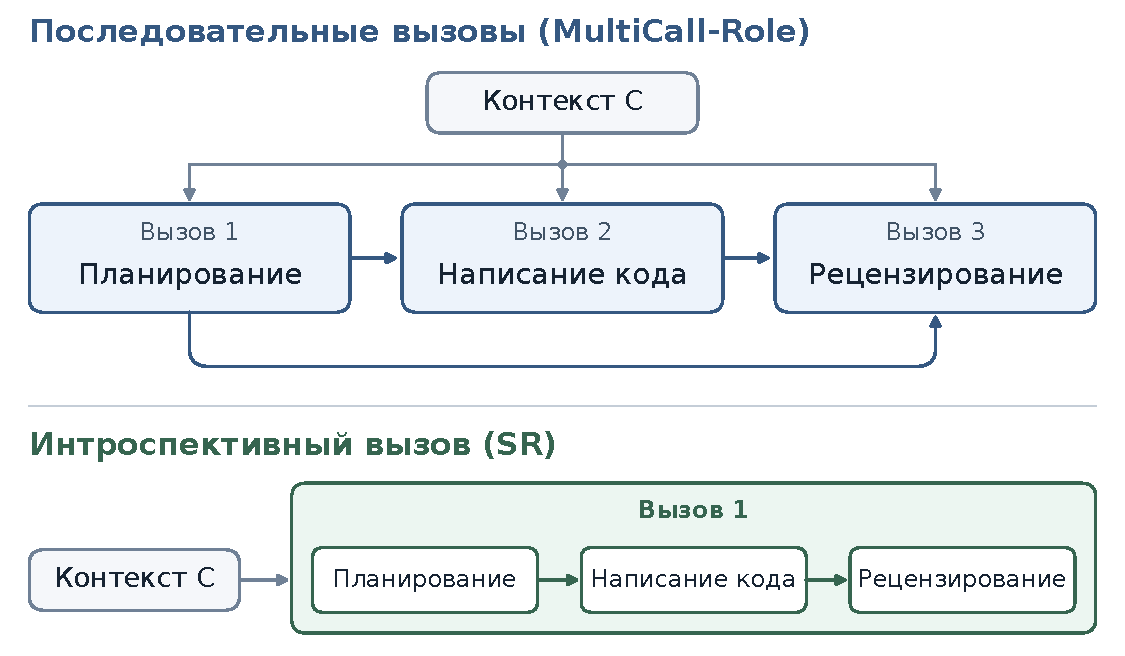
\includegraphics[width=\textwidth]{figures/context-flow.pdf}
\caption{Передача исходного контекста $C$ при трёх последовательных вызовах и~одном интроспективном. Вверху стрелки между вызовами показывают, куда передаются ответы. Внизу стрелки внутри общего блока показывают порядок действий, заданный одним запросом.}
\label{fig:context-flow}
\end{figure}
\FloatBarrier

Например, если общий контекст содержит 4\,000 токенов, три вызова получают в~сумме 12\,000 входных токенов контекста, а~интроспективный вызов получает 4\,000. Разница составляет 8\,000 токенов. Означает ли это, что с~увеличением общего контекста объединять вызовы становится выгоднее? Если остальные составляющие одинаковы, каждый дополнительный токен общего контекста увеличивает разницу на два входных токена. Чтобы оценить весь расход и~его стоимость, нужно учесть также длину инструкций и~ответов, подготовку контекста, кэширование и~возможные вызовы для исправления кода (раздел~\ref{sec:analysis}).

Что требует меньше энергии при решении одной задачи --- один вызов со всеми этапами или три вызова, каждый с~одним этапом и~повторной передачей контекста? Для ответа нужны измерения вычислительной нагрузки и~энергии всех операций, включая самую ресурсоёмкую. В~этой работе измеряется расход токенов и~оценивается их тарифная стоимость. Энергопотребление оборудования в~эти измерения не входит.

В~аналитической части сравниваемый вариант последовательных вызовов обозначен как Classical-MAS, а~в~эксперименте как \MultiCallRole{}. Каждый его вызов получает полный контекст. В~других схемах взаимодействия ролей передача данных может быть устроена иначе. Интроспективный вызов может дать более длинный ответ, рецензирование может пропустить ошибку, а~исправление может потребовать нового обращения к~модели. Поэтому экономию оцениваем вместе с~долей программ, успешно прошедших независимую проверку.

\subsection{Цель, вопросы и~задачи исследования}
Цель работы --- определить, при каких условиях один интроспективный вызов снижает расход токенов и~расчётную стоимость генерации кода по сравнению с~тремя последовательными вызовами, и~оценить изменение качества относительно этого базового варианта.

За меру качества принимаем долю программ, прошедших все тесты задачи. Обозначим эту долю в~процентах через $p_{\mathrm{SR}}$ для интроспективного вызова и~$p_{\mathrm{base}}$ для базового последовательного варианта. Разность $\Delta_Q=p_{\mathrm{SR}}-p_{\mathrm{base}}$ измеряется в~процентных пунктах. Если допустимое снижение качества заранее задано как $\delta\geq 0$ п.п., целевая граница для разности равна $-\delta$. В~проведённых сериях оцениваем разность долей и~её неопределённость. Значение $\delta$ требуется для отдельной проверки не меньшей эффективности (раздел~\ref{sec:analysis}).

Основной вопрос работы состоит в~том, \emph{когда объединение этапов снижает расход и~расчётную стоимость всех вызовов на задачу и~как при этом меняется доля успешных решений относительно базового варианта}. Расход рассматриваем с~точки зрения пользователя, который обращается к~модели через API или по подписке. В~обоих случаях число токенов характеризует объём работы с~моделью. Тарифная оценка показывает стоимость такого объёма при оплате по API. Фактическая плата за подписку определяется её условиями, а~оборудование и~энергозатраты поставщика обсуждаются отдельно (раздел~\ref{sec:limits}).

Для сравнения сформулированы четыре вопроса.
\begin{enumerate}
\item \textbf{RQ1.} Как меняется доля программ, успешно прошедших независимую проверку на тестах BigCodeBench, при переходе от трёх последовательных вызовов к~одному интроспективному?
\item \textbf{RQ2.} Как при таком переходе меняются суммарный расход входных и~выходных токенов и~расчётная стоимость обращений к~модели и~при каких условиях объединение этапов даёт экономию с~учётом подготовки контекста, ответов и~возможных исправлений?
\item \textbf{RQ3.} Как интроспективный вызов соотносится по доле программ, прошедших одни и~те же независимые тесты, с~прямым запросом и~с~многошаговой процедурой, где модель отдельно вызывается в~ролях аналитика, разработчика и~тестировщика, и~как различается расчётная стоимость интроспективного и~многошагового способов?
\item \textbf{RQ4.} Как меняются доля успешных программ, расход токенов, расчётная стоимость и~время решения, если контроллер для каждой задачи выбирает между одним и~тремя вызовами по заранее заданному требованию к~разделению работы?
\end{enumerate}

В~качестве многошагового варианта в~RQ3 используется Self-Collaboration Code Generation (SCC)~\cite{dong2023selfcollaboration}. В~этой процедуре одна модель по очереди выполняет роли аналитика, разработчика и~тестировщика. Контроллер запускает код на примерах тестировщика и~может запросить исправление. Поэтому сравнение с~SCC охватывает всю процедуру, включая внутренние проверки. Качество готового кода в~сравнении с~SCC оценивается по независимым тестам BigCodeBench (приложение~\ref{subsec:scc}).

\Needspace{7\baselineskip}
Исследование включает пять задач.
\begin{enumerate}
\item Зафиксировать содержание запросов, действия модели, формат итогового кода и~единый критерий проверки, чтобы сравнение способов вызова можно было воспроизвести на одних и~тех же задачах.
\item Вывести условия, при которых процедура с~интроспективным вызовом требует меньше токенов, чем процедура с~последовательными вызовами, с~учётом подготовки контекста и~возможных исправлений.
\item Сопоставить способы организации вызовов на одних и~тех же задачах. Добавить варианты без названий ролей, чтобы проверить, связано ли различие с~самим разделением работы или с~формулировкой инструкции.
\item Оценить качество кода по доле программ, прошедших тесты, и~проверить, как на вывод влияют разброс результатов повторных генераций и~пропуски.
\item Сравнить расход токенов и~расчётную стоимость с~учётом промежуточных ответов. Если есть незавершённые запуски, учесть и~их известные расходы.
\end{enumerate}

\emph{Доверительный интервал} показывает точность оценки разницы долей успеха. В~главном сравнении $A$ --- один интроспективный вызов SR, а~$B$ --- три последовательных вызова \MultiCallRole{}. Результат $Y_{imr}$ равен 1, если программа в~прогоне $r$ способа $m$ на задаче $i$ прошла тесты, и~0 в~случае неуспеха. Сопоставляем доли успеха за три прогона каждого способа на задачу. Усредняем разности по $n$ задачам с~шестью известными исходами и~выражаем оценку в~процентных пунктах.
\begin{formulakey}
\[
 d_i=\frac{1}{3}\sum_{r=1}^{3}(Y_{iAr}-Y_{iBr}),
 \qquad \widehat{\Delta}_Q=\frac{100}{n}\sum_{i=1}^{n}d_i.
\]
\begin{symbols}
\sym{i,\ r}{номер задачи и~номер одного из трёх прогонов}
\sym{A,\ B}{сравниваемые способы, один и~три вызова соответственно}
\sym{Y_{iAr},\,Y_{iBr}}{результаты тестов двух программ в~этом повторе, 1 при успехе и~0 при неуспехе}
\sym{d_i}{разность долей успеха на одной задаче}
\sym{n,\ \widehat{\Delta}_Q}{число задач с~полными данными и~средняя разность по ним в~процентных пунктах}
\end{symbols}
\end{formulakey}
Повторно набираем из исходной выборки 10\,000 наборов по $n$ задач. Это \emph{парный бутстрэп}~\cite{efron1986bootstrap}. В~один набор задача может попасть несколько раз. Для неё каждый раз берём разность $d_i$, рассчитанную по всем шести прогонам. Если у~$A$ на задаче прошли тесты две программы, а~у~$B$ одна, берём $d_i=2/3-1/3$. Для каждого набора пересчитываем среднюю разность. Границы интервала отсекают по 2,5\% самых низких и~самых высоких оценок. При повторении исследования примерно 95\% таких интервалов охватили бы разницу долей успеха, которую в~среднем даёт эксперимент при тех же настройках и~отборе задач. Это свойство зависит от предпосылок метода.

В~таблице~\ref{tab:scale-contrasts} четыре разности долей успеха. Сравниваем один вызов с~тремя отдельно для запросов с~названиями ролей и~для запросов с~номерами этапов. Также сравниваем названия ролей с~номерами этапов при одном и~при трёх вызовах. Чтобы охватить все четыре разности одновременно примерно с~95\%-й надёжностью, по поправке Бонферрони~\cite{nistbonferroni} строим каждый интервал Стьюдента с~уровнем $1-0{,}05/4=98{,}75\%$ (таблица~\ref{tab:precision}).

\Needspace{6\baselineskip}
Основную оценку считаем по задачам с~полными результатами. Отдельно проверяем, могли ли пропуски изменить вывод на всей тысяче задач. Для этого подставляем крайние возможные исходы вместо неизвестных. Даже самый неблагоприятный для одного вызова вариант оставляет разность положительной (раздел~\ref{subsec:missing-outcomes}).

\subsection{Интроспективный вызов и~основные результаты}
В~основном эксперименте при SR модель получала исходный контекст и~инструкции для всех трёх этапов одним запросом. На один прогон SR приходилось одно обращение к~модели. После генерации код запускал отдельный оценщик BigCodeBench. Внешние тесты давали общий критерий качества для всех способов и~выполнялись без обращения к~LLM.

В~формальном описании Hybrid-INoT из раздела~\ref{sec:method} предусмотрен дополнительный режим. Если код проваливает доступные во время работы тесты, можно передать сообщение об~ошибке модели для исправления. Такое исправление требует второго вызова, расход которого входит в~общий бюджет. В~сравнении на BigCodeBench итоговые тесты запускались после последнего ответа модели. В~разделе~\ref{sec:analysis} выведено условие экономии токенов для RQ2 с~учётом подготовки контекста, ответов и~возможных исправлений.

BigCodeBench~\cite{zhuo2024bigcodebench} содержит задачи на написание функций Python и~автоматические тесты к~ним. Две основные серии сравнивают число вызовов и~наличие названий ролей на 200 и~1\,000 задачах этого набора. В~отдельной серии на 80 задачах сравнили названия ролей и~номера этапов при одинаковых требованиях к~планированию, написанию и~проверке кода. Два способа оформления позволяют проверить это различие при записи этапов по строкам и~в~одном абзаце. Полные запросы приведены в~приложениях~\ref{app:prompt-lines} и~\ref{app:prompt-paragraph}. Проведено также сравнение с~SCC. Подготовительная серия на 40 задачах использовалась для отладки извлечения кода из ответа и~его запуска на автоматических тестах. Устройство серий и~пересечения выборок описаны в~разделе~\ref{sec:eval}.

В~расширенной серии полные данные о~расходе обоих способов доступны на 986 задачах. У~15 из них среда тестирования не прошла контроль на эталонной и~заведомо неверной программах. Расходы на этих задачах входят в~ресурсное сравнение. Для совместного сравнения использована 971 задача с~полными результатами тестов и~данными о~расходе. На этих задачах доля успехов при одном вызове выше на 2,13 процентного пункта, а~суммарная расчётная стоимость на 64,1\% ниже, чем при трёх последовательных. В~сумму входят и~расходы на программы, провалившие тесты (таблица~\ref{tab:scale-quality-cost}).

Для совместной оценки делим суммарную расчётную стоимость каждого способа на число программ, прошедших тесты. На общей выборке эта стоимость на одну успешную программу была у~интроспективного вызова ниже на 65,5\%.

В~отдельной локальной серии для RQ4 сам контроллер выбирает число вызовов по требованию к~сессии рецензента. В~этом сравнении время измерено от выбора режима до получения результата тестирования (раздел~\ref{subsec:route-pilot}).

\section{Связанные работы и~отличие предлагаемого подхода}\label{sec:related}
\subsection{Промежуточные рассуждения и~исправление ответа}
Wei и~соавторы~\cite{wei2022cot} исследовали Chain-of-Thought. Модель получает примеры, в~которых перед ответом записаны промежуточные шаги решения. На изученных арифметических, логических и~символьных задачах такие примеры повышали долю правильных ответов у~ряда крупных моделей. Это показало, что способ задания рассуждения может влиять на результат, хотя величина эффекта зависит от модели и~задачи.

В~Self-Refine Madaan и~соавторы~\cite{madaan2023selfrefine} используют одну модель для получения ответа, подготовки замечаний и~исправления. Эти операции выполняются через последовательные обращения к~модели. Reflexion Shinn и~соавторов~\cite{shinn2023reflexion} добавляет память о~прошлых ошибках: текстовую обратную связь сохраняют и~используют в~следующих попытках. Такая обратная связь может поступать как от модели, так и~из внешней среды.

ReAct Yao и~соавторов~\cite{yao2022react} чередует рассуждение с~действиями, например поиском информации. Полученное наблюдение помогает выбрать следующий шаг. Sun и~Zeng~\cite{sun2025inot} в~Introspection of Thought (INoT) задают диалог и~самопроверку с~помощью инструкции, похожей на программу. Hybrid-INoT развивает идею организации ролевых действий в~одном обращении к~модели и~дополняет её внешней проверкой кода. В~основном эксперименте изучается только объединение заданных действий. Прямое превосходство над оригинальным INoT этим сравнением не проверяется.

Turpin и~соавторы~\cite{turpin2023unfaithful} показали, что записанная цепочка рассуждений может не отражать причин ответа модели. Поэтому в~Hybrid-INoT план и~замечания рецензента служат рабочим текстом. Их полезность оценивается по итоговой программе, расходу ресурсов и~результатам независимых тестов.

\subsection{Отдельные агенты и~задачи программирования}
В~мультиагентных системах работу распределяют между взаимодействующими участниками~\cite{weiss1999,wooldridge2009}. MetaGPT~\cite{hong2023metagpt} и~ChatDev~\cite{qian2023chatdev} применяют такой подход к~разработке программ. Участники выполняют разные функции и~передают друг другу результаты. Набор инструментов и~состав контекста определяются реализацией каждой системы.

Обзоры и~исследования масштабирования обсуждают трудности согласования работы агентов~\cite{guo2024survey,qian2024scaling}. Одна из них --- расход на повторную передачу контекста и~промежуточных сообщений. Число сообщений зависит от порядка взаимодействия. При обмене между каждой парой ролей оно может расти квадратично с~числом ролей. В~последовательной цепочке сообщений существенно меньше. Поэтому затраты нужно считать для конкретного процесса.

Self-Collaboration Code Generation (SCC)~\cite{dong2023selfcollaboration} близок к~исследуемой последовательности: аналитик, разработчик и~тестировщик взаимодействуют через отдельные обращения к~модели. Для сравнения использован авторский код SCC с~изменёнными интерфейсом вызова и~числом итераций. Эти изменения описаны в~приложении~\ref{subsec:scc}. В~отличие от основного сравнения одного и~трёх вызовов, серия с~SCC оценивает процесс целиком, включая его внутренние проверки.

Для оценки кода применяются задачи разного масштаба. HumanEval~\cite{chen2021humaneval} содержит задания на написание отдельных функций. SWE-bench~\cite{jimenez2023swebench} проверяет исправления в~реальных репозиториях, а~SWE-agent~\cite{yang2024sweagent} исследует влияние интерфейса доступа к~файлам и~инструментам на их решение. В~нашей работе выбран BigCodeBench~\cite{zhuo2024bigcodebench}: задачи на создание функций Python с~использованием библиотек и~подробных требований. Его тесты позволяют сравнить программы в~одинаковых условиях. Измерения в~этой серии относятся к~отдельным функциям Python.

\subsection{Сжатие контекста и~внешние проверки}
LongLLMLingua~\cite{jiang2023longllmlingua} и~LLMLingua-2~\cite{pan2024llmlingua2} сокращают входной текст, стараясь сохранить нужную для ответа информацию. Jia и~соавторы~\cite{jia2026compression} исследуют сжатие кода при исправлении задач из репозиториев. В~основном сравнении мы передаём полный исходный контекст. Оценка методов его сжатия при передаче между вызовами выходит за рамки исследования.

Внешние инструменты проверяют программу независимо от того, насколько убедительно модель описывает своё решение. Тест выполняет код на заданных входных данных и~сверяет полученные выходные данные с~ожидаемыми. Статический анализ исследует свойства программы без её запуска. Компилятор обнаруживает нарушения правил языка и~часть несовместимостей интерфейсов. CoCoGen~\cite{bi2024cocogen} использует обратную связь компилятора для уточнения кода с~учётом проекта. Su и~McMillan~\cite{su2025static} исследуют ограничения самих языковых моделей в~задачах статического анализа. Оценщик отмечает решение как успешное, если программа проходит все выбранные тесты.

\section{Постановка задачи и~обозначения}\label{sec:problem}
\subsection{Входы, выходы и~внешние инструменты}
Условие задачи, код, документацию и~сообщения инструментов будем представлять конечными строками. Пусть $\Sigma$ --- конечный алфавит символов, а~$\Sigma^*$ --- множество конечных строк над ним. Множество $\mathcal{X}\subseteq\Sigma^*$ содержит допустимые описания заданий. Множество $\mathcal{Y}\subseteq\Sigma^*$ содержит записи решений: текст программы или набор изменений файлов в~заранее выбранном формате. Полученную запись решения будем называть \emph{кандидатом}. Проверка может обнаружить в~этом варианте программы синтаксические ошибки.

\begin{definition}[Задача программирования]
Задача $z$ --- это кортеж $(x,\mathcal{C}_0,\mathcal{Z},\mathcal{V}_z)$, где $x\in\mathcal{X}$ --- условие, $\mathcal{C}_0\in\Sigma^*$ --- исходный контекст, $\mathcal{Z}$ --- конечное множество разрешённых инструментов, а~$\mathcal{V}_z:\mathcal{Y}\to\{0,1\}$ --- фиксированное правило внешней проверки кандидата.
\end{definition}

В~$\mathcal{C}_0$ файлы, документация и~журналы ошибок записаны с~разделителями и~именами источников. Для каждого инструмента заданы формат текстового запроса, формат ответа и~предельное время выполнения. Если время истекло, инструмент возвращает специальное сообщение. Версии инструментов и~среда фиксируются. В~этой модели проверка воспроизводима: один и~тот же кандидат в~одной среде получает одинаковый результат. Случайность внешних проверок здесь не рассматривается.

Значение $\mathcal{V}_z(y)=1$ означает, что кандидат $y$ прошёл все предусмотренные проверки за отведённое время. Значение $0$ означает отрицательный результат, ошибку или превышение времени проверки. В~журнале эти причины различаются. Успех относится к~выбранному набору проверок и~не доказывает правильность программы на всех возможных входах.

Длину строки $u$ в~токенах обозначим $\len{u}$. Для всех длин используется один зафиксированный токенизатор --- правило разбиения текста на токены. В~частности, $L=\len{\mathcal{C}_0}$ --- длина исходного контекста. Символ $\bot$ означает, что процедура завершилась без кандидата. В~этом случае она возвращает этот символ и~причину остановки. В~формальной модели это неуспешное завершение процедуры. Незавершённые экспериментальные запуски с~неизвестным исходом учитываются отдельно по правилам раздела~\ref{sec:eval}.

\subsection{Случайность, ресурсы и~качество}
Представим, что одну задачу несколько раз решают одной моделью с~теми же инструкциями и~лимитами. В~одном запуске программа может пройти все тесты с~первой попытки, в~другом модель может вернуть иной код или израсходовать больше токенов. Ответы модели, обращения к~инструментам и~их результаты составляют историю запуска. Вероятность события означает, насколько часто оно происходило бы при многократном повторении процедуры в~тех же условиях. Например, событие <<программа прошла проверку>> объединяет все истории с~таким исходом.

Для процедуры $A$ обозначим итоговую программу через $Y_A$, число потраченных токенов через $T_A$, стоимость через $C_A$, а~длительность через $\ell_A$. Расход отдельного запуска включает все обращения к~модели, в~том числе подготовку контекста и~повторы. Выполнение тестов занимает время. Если оценщик сам не обращается к~модели, её токены на тестирование не расходуются.

Средний расход на \emph{одну и~ту же задачу} обозначаем $\E[T_A]$. Его оценивают средним числом токенов по повторным запускам. Вероятность успеха оценивают долей запусков, в~которых программа прошла проверку. Если процедура штатно завершилась без программы ($\bot$), это известный неуспех. Если связь со~средой прервалась и~результат теста неизвестен, запись остаётся пропуском. Усреднение результатов по \emph{разным задачам} описано в~разделе~\ref{sec:metrics}.

Для работы задаются три лимита: $B$ токенов, $B_{\$}$ денежных единиц и~$B_{\ell}$ секунд. Перед каждым платным вызовом, в~том числе вспомогательной модели, система резервирует его максимальный разрешённый расход. Если остатка бюджета недостаточно, вызов не выполняется. Каждой операции отводится не больше оставшегося общего времени. Это правило распространяется и~на подготовку контекста, и~на внешнюю проверку. При исчерпании $B_{\ell}$ работа прекращается. Если сервис не позволяет надёжно ограничить токенный расход, $B$ остаётся целевым лимитом, а~его превышение записывается отдельно.



\section{Метод Hybrid-INoT}\label{sec:method}
\subsection{Состояние и~интроспективный проход}
В~процедуре с~внешней обратной связью одна \emph{итерация} включает интроспективный вызов и~проверку полученного кода. Выполнение трёх ролевых инструкций в~одном обращении далее называем \emph{интроспективным проходом}. Если проверка обнаруживает ошибку, следующая итерация начинает новое обращение к~модели. Перед итерацией $i$ система хранит условие задачи, подготовленный контекст, историю попыток, номер итерации и~остаток токенного бюджета. Вместе эти данные образуют состояние
\begin{formulakey}
\begin{equation}
\sigma_i=(x,\widehat{\mathcal{C}}_i,\mathcal{H}_i,i,b_i).
\end{equation}
\begin{symbols}
\sym{\sigma_i}{состояние перед вызовом}
\sym{i}{номер итерации}
\sym{x}{условие задачи}
\sym{\widehat{\mathcal C}_i}{подготовленный контекст}
\sym{\mathcal H_i}{записи предшествующих попыток, включая программы, оценки и~диагностику}
\sym{b_i}{число токенов, оставшихся в~бюджете}
\end{symbols}
\end{formulakey}
Если часть истории снова передают модели, её токены учитываются в~новом вызове.

Предельное число итераций задаётся целым $I\ge1$. За один проход модель готовит целое число кандидатов $K\ge1$. Множество текстовых планов обозначим через $\Pi\subseteq\Sigma^*$.
\begin{formulakey}
Входы и~выходы трёх действий связаны следующим образом.
\nopagebreak
\begin{align}
r_{\mathrm{plan}} &: (x,\widehat{\mathcal{C}}_i,b_i)\mapsto\pi_i\in\Pi,\\
r_{\mathrm{work}} &: (\pi_i,\widehat{\mathcal{C}}_i,K)\mapsto(y_{i,1},\ldots,y_{i,K})\in\mathcal{Y}^{K},\\
r_{\mathrm{crit}} &: ((y_{i,k})_{k=1}^{K},\widehat{\mathcal{C}}_i)\mapsto(s_{i,1},\ldots,s_{i,K})\in[0,1]^K.
\end{align}
\begin{symbols}
\sym{r_{\mathrm{plan}},\,r_{\mathrm{work}},\,r_{\mathrm{crit}}}{действия планировщика, исполнителя (worker) и~рецензента (critic)}
\sym{i,\ x,\ \widehat{\mathcal C}_i,\ b_i}{номер итерации, условие задачи, её подготовленный контекст и~оставшийся бюджет}
\sym{\pi_i\in\Pi}{текст плана из множества допустимых планов}
\sym{K,\ k}{число вариантов программы в~ответе и~номер варианта от 1 до~$K$}
\sym{y_{i,k},\ \mathcal Y^K}{текст одного варианта и~множество упорядоченных списков из~$K$ вариантов}
\sym{s_{i,k}\in[0,1]}{оценка варианта рецензентом по инструкции. Более высокое значение означает более предпочтительный вариант}
\end{symbols}
\end{formulakey}
В~запросах эксперимента роли исполнителя и~рецензента помечены словами \texttt{IMPLEMENTER} и~\texttt{REVIEWER} (приложение~\ref{app:prompt-lines}).

Все три действия задаются одной инструкцией. Если из ответа нельзя извлечь план, варианты программ и~их оценки, контроллер записывает ошибку формата.

Контроллер выбирает программу с~наибольшей оценкой рецензента. Если одинаковую максимальную оценку получили несколько программ, для проверки берётся первая из них в~порядке ответа.
\begin{formulakey}
\begin{equation*}
\begin{aligned}
 k_i^\star &= \min\{k: 1\le k\le K,\ s_{i,k}=\max_{1\le j\le K}s_{i,j}\},\\
 y_i &=y_{i,k_i^\star},\\
 s_i &=s_{i,k_i^\star},
\end{aligned}
\end{equation*}
\begin{symbols}
\sym{i,\ K}{номер итерации и~число программ в~ответе}
\sym{k,\ j}{номера вариантов в~этом ответе}
\sym{k_i^\star}{номер выбранной программы}
\sym{y_{i,k},\ s_{i,k}}{программа под номером~$k$ и~её оценка рецензентом}
\sym{y_i,\ s_i}{выбранная программа и~её оценка}
\end{symbols}
\end{formulakey}
\begin{formulakey}
После запуска программы внешняя проверка возвращает три поля.
\nopagebreak
\begin{equation*}
\begin{aligned}
 v_i &= \mathcal V_z(y_i)\in\{0,1\},\\
 M_i &\in [0,1]\cup\{\mathrm{NA}\},\\
 e_i &\in\Sigma^*,
\end{aligned}
\end{equation*}
\begin{symbols}
\sym{i,\ z,\ y_i}{номер итерации, задача и~выбранная программа}
\sym{v_i,\ \mathcal V_z}{результат проверки и~правило проверки для задачи. Значение 1 означает успех, 0 означает неуспех}
\sym{M_i}{дополнительный показатель свойств кода из раздела~
ef{sec:metrics}. Метка NA означает, что показатель недоступен}
\sym{e_i,\ \Sigma^*}{сообщение о~результате и~множество допустимых текстовых строк}
\end{symbols}
\end{formulakey}

\subsection{Выбор режима работы}\label{subsec:route-rule}
Контроллер читает требования к~организации работы до первого обращения к~модели. Обычно он объединяет планирование, написание кода и~рецензирование в~одном запросе. Если условия задачи требуют разделить исполнителей или параллельно выполнять независимые подзадачи, он выбирает отдельные обращения.
\begin{formulakey}
\begin{equation}
\mathrm{RouteMode}(z)=
\begin{cases}
\mathrm{external}, & \varphi_{\mathrm{sep}}(z)=1\ \lor\ \varphi_{\mathrm{par}}(z)=1,\\
\mathrm{internal}, & \text{в остальных случаях},
\end{cases}
\end{equation}
\begin{symbols}
\sym{z}{задача вместе с~требованиями к~её выполнению}
\sym{\varphi_{\mathrm{sep}}}{признак разделения исполнителей, например требование отдельной сессии рецензента}
\sym{\varphi_{\mathrm{par}}}{признак обязательного параллельного выполнения независимых подзадач}
\sym{\lor}{логическое <<или>>. Достаточно любого из двух требований}
\sym{\mathrm{internal},\,\mathrm{external}}{один общий вызов или отдельные обращения к~модели}
\end{symbols}
\end{formulakey}
В~пилотном сравнении использован первый признак. Если в~карточке задачи явно запрошена отдельная сессия рецензента, контроллер последовательно делает три обращения, передавая между ними план и~код. В~остальных случаях он делает один вызов. Маршрут задан до генерации, выбор не требует обращения к~LLM. Все задачи пилота допускают последовательное выполнение. Измерения приведены в~разделе~\ref{subsec:route-pilot}.

\subsection{Повторные попытки и~остановка}
Ход одного запуска и~условия остановки показаны на диаграммах приложения~\ref{app:uml}. В~конфигурации с~исправлениями результат доступного во время работы теста можно передать модели в~следующем запросе. В~общий бюджет входят все обращения к~модели. Итоговые независимые тесты запускаются после завершения генерации.

При неуспехе возвращается программа с~наибольшей оценкой рецензента среди проверенных кандидатов. Отрицательный результат её внешней проверки сохраняется. Если за все попытки получены только ошибки формата, система возвращает $\bot$.

\Needspace{8\baselineskip}
\begin{proposition}[Конечность процедуры]\label{prop:termination}
Пусть $I$ конечно. Подготовка контекста, каждый вызов модели и~каждая внешняя проверка завершаются за конечное время либо прекращаются по лимиту времени. Тогда режим с~интроспективным вызовом на рисунке~\ref{fig:uml-iteration} завершается после не более чем $I$ интроспективных проходов.
\end{proposition}
\begin{proof}
Внешний цикл содержит не более $I$ итераций. На каждой выполняется конечное число операций, ограниченных по времени. При успехе или исчерпании лимита цикл завершается раньше. Следовательно, вся процедура завершается за конечное время.
\end{proof}

Конечность процедуры не означает, что оценки рецензента сходятся или что программа верна. Из условия $s_i\in[0,1]$ не следует сближение соседних оценок. Например, последовательность $0,1,0,1,\ldots$ ограничена, но разность соседних значений по модулю всегда равна единице.

Для досрочной остановки можно использовать правило $|s_i-s_{i-1}|<\varepsilon$, где $i\ge2$, а~$\varepsilon>0$ задано заранее. Оно применяется к~двум соседним проходам, из которых удалось извлечь оценки. Это практическое правило сокращения затрат: оно может завершить поиск до того, как найдена успешная программа. В~базовой конфигурации правило выключено.

\subsection{Сжатие контекста}
Сжатие --- сокращение текста, который передаётся модели. Оно может снизить расход входных токенов, но требует собственных ресурсов и~может удалить важную деталь. В~журнал записываются длина полученного текста и~затраты на само сжатие.

Обязательные части контекста включают условие, ограничения, изменяемый код и~необходимые интерфейсы. Для остальных фрагментов можно использовать оценку релевантности, например на основе LLMLingua-2~\cite{pan2024llmlingua2}. Порядок отбора и~проверка лимита показаны на рисунке~\ref{fig:uml-context} приложения~\ref{app:uml}. В~экспериментальных сравнениях модель получала контекст без сжатия.
\FloatBarrier

\section{Учёт токенов и~денежных затрат}\label{sec:analysis}
\subsection{Из чего складывается расход токенов}
Сначала посчитаем расход токенов для одной задачи. Длину её исходного контекста обозначим через $L$. Один цикл планирования, подготовки кандидатов (вариантов программы для решения задачи) и~рецензирования будем называть \emph{раундом}. Зафиксируем число основных раундов $n\ge1$ и~предположим, что оба метода выполняют их полностью. Если возможна остановка до завершения этих раундов, приведённую ниже оценку нужно проверить с~учётом фактического числа раундов.

Если после основных раундов понадобились исправления, все токены дополнительных вызовов, включая повторную передачу контекста, входят в~остаточный расход. Для последовательной процедуры он обозначается $R_{\mathrm{MAS}}$, для интроспективной ветви гибридной процедуры --- $R_{\mathrm H}$.

\Needspace{10\baselineskip}
В~сравниваемом варианте Classical-MAS один раунд содержит $m\ge1$ последовательных отдельных вызовов, каждый из которых выполняет одну роль. Каждый получает весь исходный контекст длины $L$. В~интроспективной ветви Hybrid-INoT на раунд приходится один интроспективный вызов. Длину подготовленного общего контекста в~его $i$-м вызове обозначим через $L_i$. Полный расход токенов равен сумме этих входов и~остальных затрат:
\begin{formulakey}
\begin{align}
T_{\mathrm{MAS}}&=nmL+R_{\mathrm{MAS}},\label{eq:ledger-mas}\\
T_{\mathrm{H}}&=T_{\mathrm{cmp}}+\sum_{i=1}^{n}L_i+R_{\mathrm{H}}.\label{eq:ledger-h}
\end{align}
\begin{symbols}
\sym{T_{\mathrm{MAS}},\,T_{\mathrm H}}{все входные и~выходные токены последовательной процедуры и~интроспективной ветви соответственно}
\sym{n,\ m}{число основных раундов и~число отдельных вызовов в~одном последовательном раунде}
\sym{L,\ nmL}{длина исходного контекста в~токенах и~число токенов всех передач этого контекста в~последовательных раундах}
\sym{i,\ L_i}{номер раунда и~длина подготовленного контекста для его интроспективного вызова}
\sym{T_{\mathrm{cmp}}}{токены подготовки и~сжатия контекста в~интроспективной ветви}
\sym{R_{\mathrm{MAS}},\,R_{\mathrm H}}{остальные токены соответствующего способа. Сюда входят инструкции, ответы, повторно переданные планы, модельные проверки и~все затраты на дополнительные попытки}
\end{symbols}
\end{formulakey}
Каждый токен учитывается один раз. Оба равенства относятся к~фиксированному способу вызова.

Ответы двух процедур и~их длины могут различаться. Эти различия учитываются в~$R_{\mathrm{MAS}}$ и~$R_{\mathrm{H}}$. Если отдельные роли получают только часть контекста, первое слагаемое в~\eqref{eq:ledger-mas} заменяется суммой фактически переданных длин. Таким образом, расчёт зависит от состава каждого вызова.

\subsection{Достаточное условие экономии}
Теперь рассмотрим семейство задач с~разной длиной контекста $L$. Для получения общей оценки зададим ограничения на рост расходов. Применимость этих ограничений к~конкретным моделям и~задачам требует проверки.

\Needspace{14\baselineskip}
\begin{assumption}\label{as:bounds}
Существуют постоянные $\kappa\in(0,1]$, $\gamma,\beta,c_0,c_1,d\ge0$, не зависящие от $L$, такие, что для всех задач рассматриваемого семейства выполнены ограничения:
\begin{formulakey}
\begin{align}
\E[T_{\mathrm{cmp}}]&\le\gamma L+c_0,\\
\E[L_i]&\le\kappa L+d\quad(i=1,\ldots,n),\\
\E[R_{\mathrm{H}}]-\E[R_{\mathrm{MAS}}]&\le\beta L+c_1.
\end{align}
\begin{symbols}
\sym{\E[\cdot]}{среднее по повторным запускам одной процедуры при фиксированной задаче}
\sym{L,\ i,\ n}{длина исходного контекста в~токенах, номер раунда и~число основных раундов}
\sym{T_{\mathrm{cmp}},\,\gamma,\,c_0}{расход подготовки контекста, наклон верхней границы этого расхода и~постоянная добавка в~токенах}
\sym{L_i,\,\kappa,\,d}{длина подготовленного контекста в~раунде~$i$, верхняя доля исходной длины и~добавка в~токенах на раунд, например для диагностики}
\sym{R_{\mathrm H},\,R_{\mathrm{MAS}}}{остаточные токены интроспективной и~последовательной процедур соответственно}
\sym{\beta,\,c_1}{наклон верхней границы разности остаточных расходов и~её постоянная добавка в~токенах}
\end{symbols}
\end{formulakey}
Все средние конечны. Число раундов и~число вызовов в~последовательном раунде фиксированы.
\end{assumption}

Коэффициенты ограничивают рост расходов для выбранного семейства задач. При увеличении длины контекста их значения остаются постоянными.

\Needspace{11\baselineskip}
\begin{proposition}[Условная экономия токенов]\label{prop:savings}
При предположении~\ref{as:bounds} положим
\begin{formulakey}
\begin{equation}
a=n(m-\kappa)-\gamma-\beta,\qquad b=c_0+nd+c_1,
\end{equation}
\begin{symbols}
\sym{a}{наклон нижней границы экономии, в~токенах экономии на токен исходного контекста}
\sym{b}{сумма постоянных накладных расходов в~токенах}
\sym{n,\ m}{число основных раундов и~число последовательных вызовов в~каждом}
\sym{\kappa,\,\gamma,\,\beta}{верхние коэффициенты для длины подготовленного контекста, затрат на его подготовку и~разности остаточных затрат соответственно}
\sym{c_0,\ d,\ c_1}{постоянные добавки на подготовку, на контекст каждого раунда и~на разность остальных затрат соответственно}
\end{symbols}
\end{formulakey}
\begin{formulakey}
Если $a>0$, то для любой рассматриваемой задачи с~$L>\tau_{\mathrm{bound}}=b/a$ выполняется
\nopagebreak
\begin{equation}
\E[T_{\mathrm{MAS}}]-\E[T_{\mathrm{H}}]\ge aL-b>0.
\label{eq:savings}
\end{equation}
\begin{symbols}
\sym{\E[T_{\mathrm{MAS}}]-\E[T_{\mathrm H}]}{средний расход последовательной процедуры за вычетом среднего расхода интроспективной ветви, в~токенах}
\sym{L,\ aL-b}{длина исходного контекста и~нижняя граница экономии в~токенах}
\sym{a,\,b,\,\tau_{\mathrm{bound}}}{прирост нижней границы на токен, постоянные расходы и~их отношение $b/a$, которое должна превысить длина контекста}
\end{symbols}
\end{formulakey}
\end{proposition}
\Needspace{11\baselineskip}
\begin{proof}
Из среднего расхода последовательной процедуры в~\eqref{eq:ledger-mas} вычтем средний расход интроспективной ветви в~\eqref{eq:ledger-h}. У~первой процедуры на исходный контекст затрачено $nmL$ токенов. Чтобы получить нижнюю границу разности, из этой величины вычитаем три верхние оценки из предположения~\ref{as:bounds}: на подготовку контекста, на его передачу в~$n$ раундах и~на разность прочих затрат. После приведения подобных членов коэффициент при длине контекста равен $a$, а~постоянный вычет равен $b$. Отсюда следует~\eqref{eq:savings}. Для сложения средних независимость затрат между раундами не требуется.
\end{proof}

Условие означает, что экономия на повторной передаче контекста должна расти быстрее дополнительных расходов на сжатие, ответы и~повторы. Порог $\tau_{\mathrm{bound}}$ получен из выбранных верхних оценок. Поэтому фактическая точка равенства затрат может находиться в~другом месте. При $a\le0$ знак разности затрат остаётся неопределённым в~рамках этого доказательства.

\noindent\textbf{Числовой пример.} Возьмём один раунд ($n=1$) и~три последовательных вызова ($m=3$). В~интроспективном вызове передаётся весь контекст ($\kappa=1$). Отдельной подготовки и~добавки к~длине контекста нет ($\gamma=c_0=d=0$). Допустим, что разница остальных затрат ограничена половиной исходной длины ($\beta=0{,}5$) и~постоянной добавкой $c_1=1\,000$ токенов. Подстановка даёт
\begin{formulakey}
\[
\begin{aligned}
 a &= 1(3-1)-0-0{,}5 = 1{,}5,\\
 b &= 0+1\cdot 0+1\,000=1\,000,\\
 b/a &=1\,000/1{,}5=666\tfrac{2}{3}.
\end{aligned}
\]
\begin{symbols}
\sym{a}{прирост нижней границы экономии на один токен контекста}
\sym{b}{постоянные накладные расходы в~токенах}
\sym{b/a}{порог длины исходного контекста в~токенах}
\end{symbols}
\end{formulakey}
Длина должна быть строго больше порога. Наименьшая целая длина с~гарантированной экономией в~этом примере составляет 667 токенов. При длине 4\,000 токенов нижняя граница экономии равна $1{,}5\cdot4\,000-1\,000=5\,000$ токенов. Параметры примера иллюстрируют расчёт и~заданы условно.

\subsection{Экономия с~учётом изменения качества}
Зафиксируем задачу $z$ и~настройки обеих процедур. Пусть $Q_{\mathrm{H}}$ и~$Q_{\mathrm{MAS}}$ --- вероятности успешной итоговой проверки $q$ (раздел~\ref{sec:metrics}) при случайном запуске каждой процедуры. Её скрытые тесты могут отличаться от проверки $\mathcal{V}_z$, используемой для исправлений во время работы. Если допускается потеря качества до $\delta$ процентных пунктов относительно Classical-MAS, критерий совместного учёта расхода и~качества имеет вид
\begin{formulakey}
\begin{equation}
\E[T_{\mathrm{H}}]<\E[T_{\mathrm{MAS}}],\qquad 100(Q_{\mathrm{H}}-Q_{\mathrm{MAS}})\ge -\delta.
\label{eq:joint-criterion}
\end{equation}
\begin{symbols}
\sym{\E[T_{\mathrm H}],\,\E[T_{\mathrm{MAS}}]}{средний расход в~токенах при интроспективном и~последовательном способах}
\sym{Q_{\mathrm H},\,Q_{\mathrm{MAS}}}{вероятности успеха тех же способов на независимой проверке}
\sym{100(Q_{\mathrm H}-Q_{\mathrm{MAS}}),\,\delta}{разность долей успеха и~заранее допустимое снижение, обе величины в~процентных пунктах}
\end{symbols}
\end{formulakey}
Первое неравенство следует из утверждения~\ref{prop:savings} при выполнении его предположений. Для второго неравенства нужны данные независимой проверки. При $\delta=0$ критерий требует, чтобы вероятность успеха оставалась как минимум на уровне базового способа.

Для совокупности задач обе части усредняются по одному и~тому же распределению задач. Теоретическая оценка переносится на это среднее, если её предположения и~условие на длину контекста выполняются для всех задач рассматриваемого семейства, а~средние затраты конечны.

Для формальной проверки не меньшей эффективности границу $\delta$ и~уровень доверия задают до анализа данных. Нижняя односторонняя доверительная граница разности должна быть выше $-\delta$. В~серии на 1\,000 задачах рассчитаны разность долей и~её двусторонний интервал (раздел~\ref{subsec:scale}). Протокол этой серии предусматривал сравнение долей с~нулевой разностью и~отдельный анализ расхода. Допустимое снижение качества в~протоколе этой серии не задавалось.

Применение условия экономии также требует проверить, укладываются ли число повторов и~длина сообщений об ошибках в~принятые границы расходов.

\subsection{Верхняя граница полного расхода}
Верхнюю границу полного расхода можно получить сложением лимитов отдельных вызовов. Обозначим через $T_{\mathrm{prep}}^{\max}$ предельный расход подготовки. Для одной итерации зададим пределы $P_{\max}$ входных и~$O_{\max}$ выходных токенов основной модели. Суммарный расход дополнительных языковых моделей в~этой итерации ограничим величиной $S_{\max}$. Тогда
\begin{formulakey}
\begin{equation}
T_{\mathrm{H}}\le T_{\mathrm{prep}}^{\max}+I(P_{\max}+O_{\max}+S_{\max}).
\label{eq:worst}
\end{equation}
\begin{symbols}
\sym{T_{\mathrm H},\,T_{\mathrm{prep}}^{\max}}{полный расход интроспективной ветви и~лимит подготовки в~токенах}
\sym{I}{предельное число итераций}
\sym{P_{\max},\,O_{\max},\,S_{\max}}{лимиты на вход, на ответ основной модели и~на совокупный расход вспомогательных моделей за одну итерацию, в~токенах}
\end{symbols}
\end{formulakey}
Величина $I$ ограничивает число итераций. Контекст, инструкции и~переданная история входят в~$P_{\max}$. Тексты всех $K$ кандидатов и~замечания рецензента уже учтены в~общем пределе ответа $O_{\max}$. Повторное умножение на $K$ завысило бы оценку. Каждая новая попытка занимает одну из $I$ итераций. Поэтому граница сохраняется и~в~случае, когда все попытки неуспешны.

Перед каждым вызовом система резервирует его максимальный расход из оставшегося бюджета. Если такой контроль охватывает и~подготовку, выполняется $T_{\mathrm{H}}\le B$. Для этого сервис должен технически обеспечивать заданные пределы. Скрытые токены рассуждения учитываются по счётчику сервиса. Если он неполон, соответствующий расход отмечается как частично наблюдаемый.

\subsection{Денежная стоимость}
Для расчёта денежной стоимости каждый вид токенов умножается на его цену. Пронумеруем все вызовы моделей за одну задачу индексом $j=1,\ldots,J_{\mathrm{all}}$. Число входных токенов без скидки обозначим через $p_j^{\mathrm{unc}}$, число входных токенов со скидкой за кэширование через $p_j^{\mathrm{cache}}$, а~число оплачиваемых выходных токенов через $r_j$. Кэширование позволяет повторно использовать ранее обработанный вход по правилам сервиса. Соответствующие цены за один токен обозначим через $c_j^{\mathrm{unc}}$, $c_j^{\mathrm{cache}}$, $c_j^{\mathrm{out}}$. Стоимость всех обращений равна
\begin{formulakey}
\begin{equation}
C_{\mathrm{inf}}=\sum_{j=1}^{J_{\mathrm{all}}}
\left(c_j^{\mathrm{unc}}p_j^{\mathrm{unc}}+
c_j^{\mathrm{cache}}p_j^{\mathrm{cache}}+c_j^{\mathrm{out}}r_j\right).
\label{eq:cost}
\end{equation}
\begin{symbols}
\sym{C_{\mathrm{inf}},\,j,\,J_{\mathrm{all}}}{стоимость всех обращений, номер вызова и~число вызовов для одной задачи}
\sym{p_j^{\mathrm{unc}},\,p_j^{\mathrm{cache}},\,r_j}{обычные входные, кэшированные входные и~оплачиваемые выходные токены вызова~$j$}
\sym{c_j^{\mathrm{unc}},\,c_j^{\mathrm{cache}},\,c_j^{\mathrm{out}}}{цены одного токена соответствующих трёх видов в~одной валюте}
\end{symbols}
\end{formulakey}
Величина $C_{\mathrm{inf}}$ выражает стоимость обращений к~моделям. Тариф за миллион токенов переводится в~цену одного токена делением на $10^6$. Для каждого расчёта фиксируются дата и~версия тарифа. Токены рассуждения учитываются один раз в~той категории, по которой они оплачиваются. Стоимость внешних вычислений рассчитывается отдельно.

\section{Показатели качества и~ресурсов}\label{sec:metrics}
\subsection{Успех всей процедуры и~её стоимость}
Пусть набор содержит $N$ задач, для каждой из которых назначено $R$ повторных генераций. Индексом $i$ обозначим задачу, а~индексом $r$ её повтор. В~выполненных сериях каждый повтор представлял собой новый запуск выбранного способа решения. Такой запуск включал один или несколько вызовов модели. Его номер служил для учёта запусков. Случайное состояние модели на стороне поставщика по этому номеру не задавалось, поэтому повторение запроса не гарантировало одинакового ответа.

Итоговую программу проверяет независимый оценщик. Его скрытые тесты не передаются модели. Результат проверки обозначим через $q_{ir}\in\{0,1\}$: единица соответствует успеху, ноль неуспеху. Этот результат может отличаться от результата проверки $\mathcal{V}_{z_i}$, доступной самой процедуре во время работы.

Определим долю успешных запусков $Q$, средний расход токенов $\overline{T}$ и~среднюю стоимость обращений к~моделям $\overline{C}$:
\begin{formulakey}
\begin{equation}
Q=\frac{1}{NR}\sum_{i=1}^{N}\sum_{r=1}^{R}q_{ir},\quad
\overline{T}=\frac{1}{NR}\sum_{i,r}T_{ir},\quad
\overline{C}=\frac{1}{NR}\sum_{i,r}C_{ir}.
\end{equation}
\begin{symbols}
\sym{Q}{доля запусков, в~которых программа прошла все итоговые тесты}
\sym{\overline T,\,\overline C}{средние расход токенов и~стоимость одного запуска}
\sym{N,\ R,\ NR}{число задач, число повторов каждой и~общее число запусков одного способа}
\sym{i,\ r}{номер задачи и~номер её повтора}
\sym{q_{ir}}{результат проверки программы на задаче~$i$ в~повторе~$r$, 1 при успехе и~0 при неуспехе}
\sym{T_{ir},\,C_{ir}}{все токены и~стоимость данного запуска, включая неудачные попытки}
\sym{\sum_{i,r}}{сумма по всем задачам и~всем их повторам}
\end{symbols}
\end{formulakey}
Если часть наблюдений отсутствует, вместе с~показателем сообщаем число доступных запусков и~число пропусков.

Показатели эффективности определим как
\begin{formulakey}
\begin{equation}
U_{\mathrm{tok}}=\frac{Q}{\overline{T}},\qquad
U_{\$}=\frac{Q}{\overline{C}}.
\label{eq:efficiency}
\end{equation}
\begin{symbols}
\sym{U_{\mathrm{tok}},\,U_{\$}}{число успешных запусков на токен и~на денежную единицу соответственно}
\sym{Q,\,\overline T,\,\overline C}{доля успехов, среднее число токенов и~средняя стоимость запуска}
\end{symbols}
\end{formulakey}
При положительных знаменателях $U_{\mathrm{tok}}$ показывает число успешных запусков на один затраченный токен, а~$U_{\$}$ на одну денежную единицу. Для расчёта используются суммарные успехи и~суммарные затраты всех запусков. Усреднение отдельных отношений дало бы другой показатель.

Вместе с~эффективностью приводятся доля успехов $Q$ и~расходы. Даже высокий показатель эффективности может сопровождаться неприемлемо низким качеством. Для наборов разных типов результаты сначала показываются раздельно. Веса для общего среднего выбираются до просмотра результатов.

Величина $Q$ относится к~результату всей процедуры, которая может включать несколько кандидатов или исправлений. Выражение <<успех в~пределах бюджета>> используется, когда бюджет явно задан и~контролируется. Оценка решения с~первой попытки требует отдельного расчёта. Показатель pass@1 относится к~одному сгенерированному кандидату без отбора по скрытым тестам~\cite{chen2021humaneval}.

\subsection{Дополнительные проверки и~свойства кода}
Дополнительную проверку программы можно разделить на тесты, статический анализ и~проверки безопасности. Их результаты обозначим через $t_{ir}$, $a_{ir}$ и~$u_{ir}$ соответственно. Каждый результат принимает значение $1$ при успешном прохождении проверки и~ноль при неуспехе. Доля запусков, прошедших все три вида проверки, равна
\begin{formulakey}
\begin{equation}
\mathrm{VCR}=\frac{1}{NR}\sum_{i,r}\I[t_{ir}=1\land a_{ir}=1\land u_{ir}=1].
\end{equation}
\begin{symbols}
\sym{\mathrm{VCR}}{доля запусков, в~которых программа прошла все три вида проверки}
\sym{N,\,R,\,NR}{число задач, число повторов на задачу и~общее число запусков одного способа}
\sym{i,\,r,\,\sum_{i,r}}{номер задачи, номер повтора и~сумма по всем таким парам}
\sym{t_{ir},\,a_{ir},\,u_{ir}}{результаты тестов, статического анализа и~проверок безопасности. В~каждом поле 1 означает успех, 0 означает неуспех}
\sym{\land,\,\I[\cdot]}{логическое <<и>> и~индикатор. Слагаемое равно 1, только когда все три результата равны 1}
\end{symbols}
\end{formulakey}
Для расчёта нужны заранее определённые проверки и~результаты каждого вида. Если часть проверок отсутствует, показатель по всей выборке не рассчитывается.

Для описания свойств программы введён дополнительный индекс $M$. Он объединяет четыре признака. Цикломатическая сложность характеризует ветвление программы: она равна числу независимых путей в~графе возможного выполнения команд~\cite{mccabe1976}. Остальные признаки описывают долю повторяющегося кода, плотность предупреждений анализатора и~долю документированных публичных функций.

Этот индекс характеризует измеряемые свойства текста программы. Работа Sepidband и~соавторов~\cite{sepidband2025complexity} исследует связь метрик сложности с~результатами генерации. Предлагаемые здесь веса признаков в~ней не проверялись.

Среднюю цикломатическую сложность функций одного кандидата обозначим через $\mathrm{CC}$. Долю дублирующихся строк обозначим через $\mathrm{Dup}$, число предупреждений на тысячу непустых строк через $\mathrm{Warn}$, а~долю документированных публичных функций через $\mathrm{Doc}$. Для приведения признаков к~общей шкале заранее задаются положительные масштабы $c_{\mathrm{cc}}$ и~$c_{\mathrm{warn}}$. Их выбирают на отдельном наборе. Нормированные значения вычисляются по формулам:
\begin{formulakey}
\begin{align}
\widehat{\mathrm{CC}}&=\min(1,\mathrm{CC}/c_{\mathrm{cc}}), &
\widehat{\mathrm{Warn}}&=\min(1,\mathrm{Warn}/c_{\mathrm{warn}}),\\
\widehat{\mathrm{Dup}}&=\mathrm{Dup}, &
\widehat{\mathrm{Doc}}&=\mathrm{Doc}.
\end{align}
\begin{symbols}
\sym{\mathrm{CC},\,\mathrm{Warn}}{средняя цикломатическая сложность и~число предупреждений на тысячу непустых строк}
\sym{c_{\mathrm{cc}},\,c_{\mathrm{warn}}}{положительные масштабы нормировки для сложности и~предупреждений}
\sym{\mathrm{Dup},\,\mathrm{Doc}}{доли повторяющихся строк и~документированных публичных функций}
\sym{\widehat{\mathrm{CC}},\,\widehat{\mathrm{Warn}},\,\widehat{\mathrm{Dup}},\,\widehat{\mathrm{Doc}}}{соответствующие признаки на шкале от 0 до~1. Операция $\min(1,x)$ ограничивает значение сверху единицей}
\end{symbols}
\end{formulakey}
Все четыре значения лежат в~$[0,1]$. Метод обнаружения дубликатов, список предупреждений и~критерий наличия документации фиксируются заранее. Если хотя бы один признак недоступен, например из-за отсутствия функций, индекс $M$ не вычисляется. Число таких случаев сообщается отдельно.

Индекс имеет вид
\begin{formulakey}
\begin{align}
M={}&w_{\mathrm{cc}}(1-\widehat{\mathrm{CC}})
+w_{\mathrm{dup}}(1-\widehat{\mathrm{Dup}})\notag\\
&+w_{\mathrm{warn}}(1-\widehat{\mathrm{Warn}})
+w_{\mathrm{doc}}\widehat{\mathrm{Doc}}.
\label{eq:maintainability}
\end{align}
\begin{symbols}
\sym{M}{сводная оценка свойств программы от 0 до~1}
\sym{w_{\mathrm{cc}},\,w_{\mathrm{dup}},\,w_{\mathrm{warn}},\,w_{\mathrm{doc}}}{веса сложности, дублирования, предупреждений и~документирования}
\sym{1-\widehat{\mathrm{CC}},\,1-\widehat{\mathrm{Dup}},\,1-\widehat{\mathrm{Warn}}}{вклады трёх признаков, для которых меньшие значения предпочтительны}
\sym{\widehat{\mathrm{Doc}}}{доля документированных публичных функций}
\end{symbols}
\end{formulakey}
Веса неотрицательны и~в~сумме равны единице, поэтому $M\in[0,1]$. При прочих равных индекс не уменьшается при снижении сложности, доли дубликатов и~числа предупреждений. Увеличение доли документированных функций также не уменьшает индекс. Таблица~\ref{tab:weights} содержит веса предложенной шкалы.

\begin{table}[!ht]
\caption{Предлагаемые начальные веса индекса свойств кода}
\label{tab:weights}
\centering\small\renewcommand{\arraystretch}{1.2}
\begin{tabularx}{\textwidth}{@{}lc>{\raggedright\arraybackslash}X@{}}
\toprule
Вес & Значение & Признак \\
\midrule
$w_{\mathrm{cc}}$ & 0,35 & Цикломатическая сложность \\
$w_{\mathrm{dup}}$ & 0,25 & Дублирование кода \\
$w_{\mathrm{warn}}$ & 0,20 & Предупреждения анализатора \\
$w_{\mathrm{doc}}$ & 0,20 & Наличие документации \\
\botrule
\end{tabularx}
\end{table}
\FloatBarrier

Веса выбраны для проверки чувствительности результатов. Стандарт ISO/IEC~25010:2023~\cite{iso25010} этих чисел не устанавливает. Оценки специалистов и~время сопровождения в~эксперименте не измерялись.

\begin{formulakey}
Для программы с~доступной оценкой свойств кода дополнительный балл равен
\[
S=qM^{\lambda},
\]
\begin{symbols}
\sym{S,\,q}{балл программы и~исход независимых тестов. При неуспехе $q=0$ и~балл равен нулю}
\sym{M}{сводная оценка свойств программы от 0 до~1}
\sym{\lambda}{вес этой оценки в~показателе, от 0 до~1. Исходное значение равно $0{,}5$}
\end{symbols}
\end{formulakey}
При $\lambda=0$ множитель $M^{\lambda}$ принимается равным единице, в~том числе для $M=0$.

Балл $S$ публикуется вместе с~основной долей успехов $Q$, всеми исходными компонентами и~долей кандидатов, для которых его удалось вычислить. В~пяти сериях, представленных далее, показатели $M$, $S$ и~VCR не измерялись. 

\subsection{Показатели обнаружения ошибок}
Полнота предварительной проверки $\mathrm{SCR}$ показывает, какую долю ошибочных кандидатов она выявила. Для её расчёта число отклонённых ошибочных кандидатов делится на число всех ошибочных кандидатов по независимой проверке. Вместе с~полнотой измеряется доля правильных кандидатов, которые предварительная процедура отклонила ошибочно. Эти два показателя позволяют оценить и~обнаружение ошибок, и~потерю правильных решений.

Показатель $\mathrm{RFR}$ равен доле применённых изменений, которые не были отменены за заранее установленный период. Для его расчёта нужны наблюдения за использованием программ после внесения изменений. Один запуск HumanEval таких данных не даёт.

Если в~выборке нет ошибочных кандидатов или применённых изменений, соответствующий знаменатель равен нулю. В~таком случае доля не определена. Это состояние сохраняется в~отчёте отдельно от нулевого значения измеренного показателя.


Показатели SCR и~RFR также не измерялись в~проведённых сериях.

\section{Проведённые эксперименты и~результаты}\label{sec:eval}
\subsection{Условия сравнения}
Для основных сравнений выбран BigCodeBench v0.1.4 в~режиме \texttt{instruct full}~\cite{zhuo2024bigcodebench}. В~каждой задаче модель получает требования к~функции Python и~должна вернуть законченную программу. После получения готовой программы её проверяют исходными тестами набора. Во время работы модель не видит эти тесты, эталонное решение и~результаты итоговой проверки.

Основное сравнение проверяет, что меняется при переходе от последовательных вызовов к~одному вызову. Дополнительные варианты без названий ролей позволяют проверить, связан ли результат с~распределением действий между вызовами или с~ролевыми словами в~запросе. Планирование, написание кода и~рецензирование можно обозначить нейтрально, как этапы 1, 2 и~3, или назвать ролями планировщика, исполнителя и~рецензента. Все три инструкции можно передать одним запросом или распределить между тремя последовательными обращениями. Получаются четыре условия. К~ним добавлен прямой запрос без предписанных этапов, чтобы проверить, нужны ли эти этапы вообще. Все пять условий представлены в~таблице~\ref{tab:design}.

\begin{table}[htbp]
\caption{Условия основного сравнения}
\label{tab:design}
\centering\small\renewcommand{\arraystretch}{1.18}
\begin{tabularx}{\textwidth}{@{}lc>{\raggedright\arraybackslash}p{2.2cm}>{\raggedright\arraybackslash}X@{}}
\toprule
Код & Вызовы & Обозначения & Предписанные действия \\
\midrule
D & 1 & Без этапов & Сразу подготовить программу. \\
SN & 1 & Этапы 1, 2, 3 & Составить план, написать код, проверить и~исправить его по требованиям. \\
SR & 1 & Названия ролей & Планировщик, исполнитель и~рецензент заданы в~одном вызове. \\
MN & 3 & Этапы 1, 2, 3 & Те же действия в~последовательных вызовах. \\
\MultiCallRole{} & 3 & Названия ролей & Планировщик, исполнитель и~рецензент заданы в~трёх отдельных вызовах. \\
\botrule
\end{tabularx}
\end{table}
\FloatBarrier

В~условиях SN, SR, MN и~\MultiCallRole{} формулировки самих действий совпадают. При трёх вызовах каждый получает полный текст задачи и~все предыдущие видимые ответы. Поэтому переход к~трём вызовам одновременно добавляет повторный контекст, промежуточные сообщения и~отдельную генерацию на каждом этапе. Эксперимент оценивает результат такого разделения работы. Определить вклад каждого из этих изменений по отдельности он не позволяет.

Условие SR соответствует интроспективному вызову с~названиями ролей. В~условии \MultiCallRole{} те же три действия с~названиями ролей распределены между последовательными вызовами. Итоговая программа в~обоих случаях проверяется тестами. Сжатие контекста, автоматический выбор числа вызовов и~исправление по результатам внешних тестов в~этом сравнении не используются. Оригинальный INoT также не воспроизводится целиком: исследуется общий для подходов принцип объединения действий внутри одного вызова.

В~первых трёх сериях BigCodeBench использовалась модель с~идентификатором \texttt{gpt-5.4-mini}, в~двух остальных сериях BigCodeBench --- \texttt{gpt-5.6-luna}. Уровень рассуждения во всех пяти сериях BigCodeBench задан как \texttt{medium}. Запросы отправлялись через Codex CLI 0.153.4 с~доступом по подписке. Каждый вызов создавал новую сессию без пользовательских инструкций и~файлов проекта. В~условиях D, SN, SR, MN и~\MultiCallRole{} инструменты были отключены. Внутренние проверки метода SCC описаны в~приложении~\ref{subsec:scc}.

Повторы нужны, потому что одна модель может дать разные программы на один и~тот же запрос. Каждый повтор представлял собой новую генерацию для той же задачи и~условия. Предыдущая программа при этом не исправлялась, а~лучший ответ по скрытым тестам не выбирался. Управление случайным состоянием модели на стороне поставщика не было подтверждено. Общий жёсткий предел выходных токенов не задавался. На один вызов отводилось 180 секунд в~сериях на 40 и~200 задачах и~600 секунд в~сериях на 80 и~1\,000 задачах. Сетевой сбой или превышение времени отмечались как незавершённый запуск. Качество отсутствующей программы оставалось неизвестным.

Основная генерация на 1\,000 задачах проходила 8--11 сентября 2026 года по UTC. Конечные записи выбранных запусков SCC относятся к~11--13 сентября, а~первое сравнение на 200 задачах выполнено 8 сентября. Даты в~именах архивных папок служат идентификаторами архивов и~не всегда совпадают с~датами выполнения. Позднейшие уточнения анализа, включая добавления 3 октября, основаны на этих же сохранённых результатах.

\subsection{Пять серий на BigCodeBench}
Единица плана эксперимента, далее \emph{назначение}, задаёт одну задачу, одно условие и~один повтор. Например, пять условий с~тремя повторами на 1\,000 задачах дают 15\,000 назначений. Таблица~\ref{tab:series} разделяет запланированные генерации, полученные программы и~программы с~доступной оценкой качества.

\begin{table}[htbp]
\caption{Объём пяти серий на BigCodeBench}
\label{tab:series}
\centering\small\renewcommand{\arraystretch}{1.15}
\begin{tabularx}{\textwidth}{@{}>{\raggedright\arraybackslash}Xrrrr@{}}
\toprule
Серия & Задачи & Назначено & Получено & Оценено \\
\midrule
Отладочная & 40 & 400 & 400 & 390 \\
Первое сравнение & 200 & 1\,000 & 996 & 963 \\
Проверка оформления & 80 & 320 & 320 & 316 \\
Расширенное сравнение & 1\,000 & 15\,000 & 14\,961 & 14\,736 \\
Сравнение с~SCC & 956 & 6\,000 & 5\,595 & 5\,503 \\
\botrule
\end{tabularx}
\end{table}
\FloatBarrier

На 40 задачах отладили весь цикл: извлекали из ответа модели программу на Python, запускали её в~изолированной среде на тестах BigCodeBench и~записывали, прошла ли она тесты. В~серии было пять условий по два повтора. Её результаты приведены отдельно от основных сравнений токенного расхода и~качества. Первое основное сравнение проводилось на 200 других задачах: пять условий по одной новой генерации. Задачи выбирались из случайной перестановки допустимых идентификаторов. Начальное состояние генератора Python было равно 20260908. Если контроль среды выявлял проблему, задача сохранялась в~плане и~не заменялась более удобной.

На 80 новых задачах сравнили два способа записи инструкций внутри одного вызова. В~первом каждое действие начиналось с~новой строки и~метки в~квадратных скобках (приложение~\ref{app:prompt-lines}). Во втором те же действия шли подряд в~одном абзаце, с~двоеточием после каждой метки (приложение~\ref{app:prompt-paragraph}). В~каждом формате были две версии: с~метками \texttt{PLANNER}, \texttt{IMPLEMENTER}, \texttt{REVIEWER} и~с~нейтральными метками \texttt{STAGE 1}, \texttt{STAGE 2}, \texttt{STAGE 3}. Обе версии поручали модели составить план, написать функцию и~проверить собственный код. Внешние тесты оценивали готовую программу, поэтому по результатам можно сравнивать формулировки запроса, а~не работу каждого этапа по отдельности. Четыре сочетания дали 320 программ. Эти 80 задач не пересекаются с~отладочными 40 и~первыми 200.

Расширенная серия включала 1\,000 задач: прежние 200 и~ещё 800. Для каждой задачи и~каждого из пяти условий заранее назначено по три новые генерации. В~протоколе это число выбрано, чтобы сохранить охват 1\,000 задач в~пределах бюджета. Вариант с~пятью повторами требовал бы 25\,000 назначений вместо 15\,000. Оптимальность именно трёх повторов не установлена. Это число не гарантирует заданной точности. Их результаты усредняются внутри задачи, а~полученная точность оценивается доверительными интервалами. Старые программы не использовались. Таким образом, увеличились число задач и~число повторов, а~модель mini была заменена на Luna. Сопоставлять серии как проверку только одного из этих изменений нельзя.

Для сравнения с~SCC выбраны первые 2\,000 сочетаний «задача--повтор» из случайно перемешанного порядка. Каждому сочетанию назначены SN, SR и~SCC, всего 6\,000 запусков. Эти сочетания охватывают 956 задач из расширенной серии: у~212 задач выбран один повтор, у~444 --- два, у~300 --- три. Исходный план на 9\,000 назначений был сокращён после начала генерации, но до просмотра качества SCC. План и~поправка сохранены. Во всех пяти сериях вместе встречается 1\,120 разных идентификаторов BigCodeBench. Суммировать размеры пересекающихся выборок было бы неверно.

\subsection{Проверка программ и~работа с~пропусками}\label{subsec:missing-outcomes}
Прежде чем оценивать ответы модели, для каждой задачи проверяли эталонную и~заведомо неверную программы. Задача включалась в~анализ качества, если эталон проходил тесты, а~неверная программа отклонялась. Такой контроль помогает отделить ошибку ответа от проблемы окружения. Программы исполнялись штатным оценщиком BigCodeBench в~изолированном контейнере без сети. Исходные тесты не менялись под ответы модели. Для каждой программы сохранялись результат, сообщения проверяющего и~связь с~назначением.

Доля успехов равна числу программ, прошедших все тесты, делённому на число программ с~известной оценкой. Оценка могла отсутствовать по двум причинам: генерация не завершилась либо среда не прошла контроль на этой задаче. Эти случаи записывались раздельно и~исключались из расчёта доли успехов по известным исходам. Программы, которые удалось проверить и~которые не прошли тесты, оставались в~анализе как неуспешные. Поэтому исключение неизвестных результатов не означает исключения ошибочного кода. Известные расходы незавершённых запусков сохранялись. Отсутствующий счётчик токенов отмечался как неизвестный.

Сравнение двух методов строилось на общих задачах. В~расширенной серии для основной оценки требовались все три результата в~обоих условиях. Сначала три повтора усреднялись внутри задачи, затем вычислялась разность между условиями. Итог представлял собой среднее этих разностей с~одинаковым весом каждой задачи. Поэтому три повтора не считались тремя независимыми задачами, а~число доступных пар могло различаться между сравнениями.

Четыре сравнения качества заданы заранее: SR с~SN, \MultiCallRole{} с~MN, MN с~SN и~\MultiCallRole{} с~SR. В~серии на 200 задачах применён точный двусторонний критерий Мак-Немара. В~серии на 1\,000 задачах использованы двусторонние парные $t$-тесты для средних по задачам. Решения принимались с~поправкой Холма~\cite{holm1979}. При предпосылках тестов она ограничивает вероятность хотя бы одного ложного положительного вывода в~этом семействе величиной 0,05.

Рядом с~оценками приведены описательные 95\%-е интервалы. Для их расчёта 10\,000 раз выбирались с~возвращением целые задачи со всеми повторами. Такой бутстрэп показывает неопределённость оценки, сохраняя связь повторов одной задачи. Эти интервалы не учитывают четыре проверки одновременно. Решение о~значимости принимается по тестам с~поправкой Холма.

Основная оценка использует задачи с~известными исходами. Чтобы проверить устойчивость вывода на всей назначенной выборке, дополнительно находим крайние возможные значения средней разности. Пусть $D$ --- разность числа известных успехов способов $A$ и~$B$, $U_A$ и~$U_B$ --- числа прогонов без оценки, а~$N$ --- число назначенных прогонов на способ. Нижняя граница равна $100(D-U_B)/N$ п.п. Она получается, если все неизвестные исходы $B$ окажутся успехами, а~все неизвестные исходы $A$ --- неуспехами. При обратном распределении получается верхняя граница $100(D+U_A)/N$. Минимум и~максимум наблюдавшихся исходов характеризуют разброс отдельных наблюдений. По рассчитанным границам видно, насколько пропуски могут сдвинуть среднюю разность на всех назначенных задачах.

Исходный план расширенной серии был сохранён до начала её генерации, а~контрольные проверки проведены до просмотра качества ответов. Это локальная фиксация протокола. Внешняя предварительная регистрация исследования не проводилась. После прерываний разрешалось продолжать только назначения, в~которых ещё не начался ни один вызов. Начатый неудачный запуск не заменялся новой попыткой в~той же ячейке. Порядок назначений перемешивался, но фактическое время завершения зависело также от параллельного выполнения и~сбоев.

\subsection{Качество на 1\,000 задачах}\label{subsec:scale}
Из 15\,000 назначений завершилось 14\,961. 39 остались незавершёнными. Контроль среды позволил оценивать качество на 985 задачах. В~результате известны 14\,736 исходов, а~264 остаются неизвестными из-за незавершённой генерации или непригодности среды. Таблица~\ref{tab:scale-quality} показывает результат каждого условия. Последний столбец рассчитан от числа оценённых программ в~той же строке.

\begin{table}[htbp]
\caption{Качество в~расширенной серии: исходы отдельных генераций}
\label{tab:scale-quality}
\centering\small\renewcommand{\arraystretch}{1.15}
\begin{tabular}{@{}lrrrr@{}}
\toprule
Условие & Получено & Оценено & Успехов & Успех, \% \\
\midrule
D & 2\,996 & 2\,951 & 1\,611 & 54,59 \\
SN & 2\,998 & 2\,953 & 1\,604 & 54,32 \\
SR & 2\,997 & 2\,952 & 1\,581 & 53,56 \\
MN & 2\,983 & 2\,938 & 1\,471 & 50,07 \\
\MultiCallRole{} & 2\,987 & 2\,942 & 1\,514 & 51,46 \\
\botrule
\end{tabular}
\end{table}
\FloatBarrier

Каждому условию было назначено 3\,000 генераций. Доступные исходы в~строках различаются, поэтому простое вычитание процентов из таблицы~\ref{tab:scale-quality} не даёт парной оценки. В~таблице~\ref{tab:scale-contrasts} разности рассчитаны на одних и~тех же задачах с~полными повторами. В~последних двух строках показано «один вызов минус три»: положительная разность означает преимущество одного вызова. Перемена знака относительно исходной записи сравнения не меняет двусторонний тест. Разность выражена в~процентных пунктах, сокращённо п.п.

\begin{table}[htbp]
\caption{Парные различия качества на 1\,000 задачах}
\label{tab:scale-contrasts}
\centering\small\renewcommand{\arraystretch}{1.2}
\begin{tabular}{@{}lrrrr@{}}
\toprule
Сравнение & Задачи & Разность, п.п. & 95\% интервал & $p$ Холма \\
\midrule
SR $-$ SN & 982 & $-0{,}75$ & $[-1{,}97;+0{,}44]$ & 0,23575 \\
\MultiCallRole{} $-$ MN & 964 & $+1{,}35$ & $[+0{,}17;+2{,}56]$ & 0,05986 \\
SN $-$ MN & 968 & $+4{,}17$ & $[+2{,}75;+5{,}65]$ & $1{,}34\cdot10^{-7}$ \\
SR $-$ \MultiCallRole{} & 971 & $+2{,}13$ & $[+0{,}82;+3{,}43]$ & 0,00445 \\
\botrule
\end{tabular}
\end{table}
\FloatBarrier

Доля программ, прошедших тесты, у~интроспективного вызова SR была на 2,13 процентного пункта выше, чем у~трёх последовательных вызовов \MultiCallRole{}. Для нейтральных инструкций разность между SN и~MN составила 4,17 пункта в~пользу SN. Оба результата проходят поправку Холма. Знак сохраняется даже при заполнении всех пропусков в~пользу трёх вызовов. По всей тысяче задач крайние границы равны $[+0{,}30;+3{,}83]$ пункта для SR минус \MultiCallRole{} и~$[+2{,}37;+6{,}00]$ для SN минус MN.

Сами названия ролей не дали подтверждённого улучшения. Различие SR и~SN статистически незначимо. Для \MultiCallRole{} минус MN оценка положительна, но скорректированное $p=0{,}05986$ превышает 0,05. Здесь описательный интервал не пересекает ноль, однако он не учитывает одновременную проверку четырёх гипотез. Этот пример показывает, зачем различать интервал отдельной оценки и~решение с~поправкой. При этом отсутствие значимости оставляет возможность небольшого эффекта.

\subsection{Проверки устойчивости основного результата}
После основного анализа выполнено несколько дополнительных проверок на сохранённых данных. Они помогают понять границы вывода, но не меняют четыре заранее заданных теста и~не добавляют новых генераций.

Сначала для тех же четырёх разностей построены более строгие интервалы, учитывающие их совместную оценку. Каждый интервал Стьюдента имеет уровень 98,75\%. Правило Бонферрони даёт приблизительное совместное покрытие не менее 95\% при предпосылках анализа по задачам. Интервалы показаны в~таблице~\ref{tab:precision}. Оба различия между одним и~тремя вызовами остаются положительными. Для названий ролей интервалы включают ноль и~допускают небольшой выигрыш: до 0,83 пункта при одном вызове и~до 2,90 при трёх.

\begin{table}[htbp]
\caption{Дополнительные интервалы с~учётом четырёх сравнений}
\label{tab:precision}
\centering\small
\begin{tabular}{@{}lrr@{}}
\toprule
Сравнение & Задачи & 98,75\% интервал, п.п. \\
\midrule
SR $-$ SN & 982 & $[-2{,}32;+0{,}83]$ \\
\MultiCallRole{} $-$ MN & 964 & $[-0{,}20;+2{,}90]$ \\
SN $-$ MN & 968 & $[+2{,}29;+6{,}04]$ \\
SR $-$ \MultiCallRole{} & 971 & $[+0{,}46;+3{,}80]$ \\
\botrule
\end{tabular}
\end{table}
\FloatBarrier

Затем результаты разделены по времени генерации. Первый завершённый сеанс содержит 5\,551 программу, последующие --- 9\,410. В~каждом периоде сопоставлялись только повторы с~известными результатами обоих методов. Разности усреднялись сначала внутри задачи, затем по задачам. Таблица~\ref{tab:temporal} показывает все четыре сравнения. Оценки преимущества одного вызова положительны в~обоих периодах. Однако ранний интервал SR минус \MultiCallRole{} включает ноль, то есть данных этого среза недостаточно для уверенного вывода о~знаке различия. Периоды пересекаются по задачам и~не являются независимыми повторениями эксперимента. Такая проверка также не исключает изменений модели у~поставщика.

\begin{table}[htbp]
\caption{Различия качества в~разные периоды генерации}
\label{tab:temporal}
\centering\small\setlength{\tabcolsep}{4pt}
\begin{tabular}{@{}llrrl@{}}
\toprule
Сравнение & Период & Задачи & \shortstack{Пары\\повторов$^*$} & \shortstack{Разность, п.п.\\{}[95\% интервал]} \\
\midrule
SR $-$ SN & Первый & 740 & 1\,096 & $-1{,}42\;[-3{,}54;+0{,}74]$ \\
 & Поздние & 936 & 1\,855 & $-0{,}66\;[-2{,}23;+0{,}91]$ \\
\MultiCallRole{} $-$ MN & Первый & 736 & 1\,090 & $+0{,}79\;[-1{,}40;+2{,}99]$ \\
 & Поздние & 934 & 1\,844 & $+1{,}41\;[-0{,}11;+2{,}93]$ \\
SN $-$ MN & Первый & 737 & 1\,092 & $+4{,}27\;[+1{,}99;+6{,}56]$ \\
 & Поздние & 934 & 1\,846 & $+4{,}46\;[+2{,}61;+6{,}37]$ \\
SR $-$ \MultiCallRole{} & Первый & 738 & 1\,092 & $+2{,}06\;[-0{,}14;+4{,}27]$ \\
 & Поздние & 934 & 1\,849 & $+2{,}37\;[+0{,}77;+4{,}00]$ \\
\botrule
\end{tabular}
\par\smallskip\raggedright\footnotesize $^*$Число пар повторов с~результатами обоих методов. Интервалы описательные, получены 10\,000 выборками целых задач, PCG64, начальное состояние 20261003.
\end{table}
\FloatBarrier

Ещё одна проверка учитывает историю выборки. Из 1\,000 задач 200 уже встречались в~ранней серии, а~800 использовались впервые. В~таблице~\ref{tab:subgroups} эти части рассмотрены отдельно. Преимущество одного вызова сохраняется на 800 новых идентификаторах: 4,17 пункта при нейтральных инструкциях и~2,35 при ролевых. Следовательно, основной результат не определяется только прежними 200 задачами. Все программы, включая ответы на прежние задачи, были сгенерированы заново.

\begin{table}[htbp]
\caption{Различия качества на прежних и~новых задачах}
\label{tab:subgroups}
\centering\small\setlength{\tabcolsep}{5pt}
\begin{tabular}{@{}llrl@{}}
\toprule
Сравнение & Выборка & Задачи & \shortstack{Разность, п.п.\\{}[95\% интервал]} \\
\midrule
SR $-$ SN & Прежние 200 & 194 & $-1{,}03\;[-3{,}78;+1{,}72]$ \\
 & Новые 800 & 788 & $-0{,}68\;[-2{,}07;+0{,}72]$ \\
\MultiCallRole{} $-$ MN & Прежние 200 & 190 & $+1{,}93\;[-0{,}70;+4{,}56]$ \\
 & Новые 800 & 774 & $+1{,}21\;[-0{,}13;+2{,}58]$ \\
SN $-$ MN & Прежние 200 & 192 & $+4{,}17\;[+0{,}87;+7{,}64]$ \\
 & Новые 800 & 776 & $+4{,}17\;[+2{,}58;+5{,}84]$ \\
SR $-$ \MultiCallRole{} & Прежние 200 & 190 & $+1{,}23\;[-1{,}23;+3{,}68]$ \\
 & Новые 800 & 781 & $+2{,}35\;[+0{,}81;+3{,}88]$ \\
\botrule
\end{tabular}
\end{table}
\FloatBarrier

Наконец, проверено сходство самих задач. Для инструкций сравнивались множества последовательностей из пяти слов после удаления служебного заключительного абзаца и~приведения к~одному регистру. Мера Жаккара равна числу общих элементов, делённому на число разных элементов в~объединении двух множеств. Инструкции связывались при значении не ниже 0,70. Отдельно проверялись пороги 0,50 и~0,90.

Объединённое правило также учитывало точные совпадения инструкций после нормализации пробелов, совпадающую структуру эталонного кода без строк документации и~близкие наборы имён и~литералов кода. Для последнего признака требовалось не менее 20 вхождений идентификаторов в~каждой программе, мера Жаккара не ниже 0,80 и~её вариант с~учётом повторений не ниже 0,70. Связи строились по всем 1\,140 задачам BigCodeBench. Задачи, связанные напрямую или через промежуточные задачи, объединялись в~группы. После ограничения на выбранную тысячу получилось 992 группы.

При повторной выборке целых групп с~сохранением весов задач интервалы для SR минус SN и~\MultiCallRole{} минус MN составили $[-1{,}99;+0{,}47]$ и~$[+0{,}14;+2{,}60]$ пункта. Для SN минус MN и~SR минус \MultiCallRole{} они равны $[+2{,}72;+5{,}69]$ и~$[+0{,}79;+3{,}44]$. Использованы 10\,000 выборок, PCG64 и~начальное состояние 20260911. Направление основного результата сохранилось при таком учёте сходства. Протокол этой проверки записан 11 сентября, уже во время генерации. Проверка охватывает заданные виды сходства. Она не устанавливает независимость всех задач или отсутствие этих задач в~обучающих данных модели.

\subsection{Сравнение с~прямым запросом}
Прямой запрос D даёт ориентир для оценки всех дополнительных этапов. Его парные сравнения в~таблице~\ref{tab:direct} выполнены после основного анализа и~носят разведочный характер. Они не входят в~семейство четырёх тестов с~поправкой Холма.

\begin{table}[htbp]
\caption{Разведочные сравнения качества прямого запроса}
\label{tab:direct}
\centering\small
\begin{tabular}{@{}lrrr@{}}
\toprule
Сравнение & Задачи & Разность, п.п. & 95\% интервал \\
\midrule
D $-$ SN & 980 & $+0{,}27$ & $[-0{,}88;+1{,}43]$ \\
D $-$ SR & 979 & $+0{,}95$ & $[-0{,}17;+2{,}11]$ \\
D $-$ MN & 966 & $+4{,}59$ & $[+2{,}97;+6{,}18]$ \\
D $-$ \MultiCallRole{} & 970 & $+3{,}20$ & $[+1{,}82;+4{,}64]$ \\
\botrule
\end{tabular}
\end{table}
\FloatBarrier

Различия D с~одним нейтральным или ролевым вызовом невелики, а~оба интервала включают ноль. Это оставляет неопределённость относительно их порядка и~не доказывает равенства. По сравнению с~тремя вызовами наблюдаемая доля успехов D выше на 3,20--4,59 пункта. Поэтому объединение этапов полезно оценивать и~относительно простого прямого запроса: SR нельзя считать лучшим из всех пяти условий только по его преимуществу над \MultiCallRole{}.

В~сравнении с~многошаговой процедурой SCC разность долей успеха SCC и~SR на 883 задачах с~общими доступными повторами составила $-2{,}68$ процентного пункта. Интервал, учитывающий все неизвестные исходы на 941 пригодной задаче, допускает оба направления эффекта. На 896 задачах с~полными парными счётчиками расчётная стоимость SCC была в~3,14 раза выше. Реализация и~полный анализ приведены в~приложении~\ref{subsec:scc}.

\subsection{Расход токенов и~расчётная стоимость}
В~расход включены входы и~выходы всех вызовов, в~том числе повторный контекст и~промежуточные ответы. Кэшированные токены уже входят в~общий вход, а~токены рассуждения --- в~выход. Повторно они не прибавляются.

Денежная оценка переводит эти счётчики в~стоимость по сохранённым тарифам программного интерфейса сервиса, или API. За миллион обычных входных, кэшированных входных и~выходных токенов использованы соответственно 0,75 / 0,075 / 4,50 доллара для mini и~0,20 / 0,02 / 1,20 доллара для Luna. Это фиксированные коэффициенты расчёта. Поскольку эксперимент выполнен через подписку, полученные суммы не являются фактическими платежами за API или стоимостью подписки. Время исследователя и~вычисления оценщика в~них не включены.

Ресурсы сравниваются на задачах со всеми тремя повторами и~известными счётчиками обоих методов. Сначала вычисляются средние внутри задач, затем средние по общему набору задач. Их отношение приведено в~таблице~\ref{tab:scale-resources}. Например, значение 2,780 для \MultiCallRole{}/SR означает, что три последовательных вызова имеют в~2,780 раза большую тарифную оценку, чем один интроспективный вызов. Наборы полных пар для качества и~ресурсов могут различаться.

\begin{table}[htbp]
\caption{Отношения ресурсов: три вызова к~одному}
\label{tab:scale-resources}
\centering\small\renewcommand{\arraystretch}{1.2}
\begin{tabular}{@{}lrrrr@{}}
\toprule
Сравнение & Задачи & Токены & API-оценка & Без скидки за кэш \\
\midrule
MN / SN & 983 & 3,078 & 2,672 & 2,777 \\
\MultiCallRole{} / SR & 986 & 3,090 & 2,780 & 2,867 \\
\botrule
\end{tabular}
\end{table}
\FloatBarrier

Три последовательных вызова \MultiCallRole{} потребовали в~3,09 раза больше токенов и~в~2,78 раза больших расчётных затрат, чем один интроспективный вызов SR. В~обратном сравнении SR использовал \textbf{на 67,6\% меньше токенов}, чем \MultiCallRole{}. Описательный 95\%-й интервал отношения затрат \MultiCallRole{}/SR равен $[2{,}74;2{,}82]$, а~MN/SN --- $[2{,}63;2{,}71]$. Преимущество одного вызова по расчётным затратам сохраняется и~при одинаковой цене всего входа, без скидки на кэш.

Абсолютная разница помогает оценить практический масштаб этих отношений. На полных ресурсных парах три нейтральных вызова добавляют в~среднем 8\,582 токена на программу по сравнению с~одним, а~три ролевых --- 8\,510. В~обоих случаях разница тарифных оценок составляет \textbf{примерно 1,60 доллара на 1\,000 генераций}. Для этих коротких задач большое относительное различие соответствует небольшой денежной сумме по использованным тарифам. Время измерялось отдельно в~локальном пилоте (раздел~\ref{subsec:route-pilot}).

Известная тарифная оценка всех завершённых кандидатов пяти условий основной серии составляет 23,07 доллара. Известные этапы незавершённых запусков добавляют около 0,03 доллара, всего 23,10 доллара. Счётчики 32 начатых этапов недоступны и~в~сумму не входят. Эти общие суммы показывают масштаб исследования. Сравнение условий опирается на полные пары, чтобы сопоставлять расходы на одном и~том же наборе задач. Такое ограничение само по себе не устраняет возможное смещение из-за пропусков.

Названия ролей меняют ресурсы заметно слабее. Отношение тарифных оценок SR/SN равно 0,939 на 997 задачах, \MultiCallRole{}/MN --- 0,978 на 979. Это описательные различия, которые нужно рассматривать вместе с~неопределённостью качества. Длина контекста отдельно не изменялась, поэтому порог из утверждения~\ref{prop:savings} по этой серии не оценивался.

\subsection{Сопоставление качества и~расхода на общих задачах}
Из 986 задач с~полными данными о~расходе 15 не прошли контроль тестовой среды. Для сравнения качества и~расходов вместе используем 971 задачу, для которой известны исходы тестов, счётчики токенов и~расчётная стоимость всех трёх прогонов каждого способа. В~общий расход входят все прогоны из этой выборки, включая программы, провалившие тесты. Таблица~\ref{tab:scale-quality-cost} показывает оба показателя по одному и~тому же набору задач.

\begin{table}[htbp]
\caption{Качество и~расходы на общей выборке из 971 задачи}
\label{tab:scale-quality-cost}
\centering\small\renewcommand{\arraystretch}{1.18}
\begin{tabular}{@{}lrr@{}}
\toprule
Показатель & SR & \MultiCallRole{} \\
\midrule
Число прогонов & 2\,913 & 2\,913 \\
Число программ, прошедших тесты & 1\,562 & 1\,500 \\
Доля успешных программ, \% & 53,62 & 51,49 \\
Токенов на прогон, в~среднем & 4\,070 & 12\,578 \\
Расчётная стоимость всех прогонов, долл. & 2,60695 & 7,25753 \\
Расчётная стоимость на успешную программу, долл. & 0,001669 & 0,004838 \\
\botrule
\end{tabular}
\end{table}
\FloatBarrier

Последняя строка --- суммарная расчётная стоимость, делённая на число успешных программ, или $1/U_{\$}$ из формулы~\eqref{eq:efficiency}. Если средняя стоимость прогона и~доля успехов уменьшатся в~одинаковой пропорции, стоимость на успешную программу останется прежней. В~этой выборке SR повысил долю успехов на 2,13 процентного пункта, а~\textbf{стоимость на успешную программу снизилась на 65,5\%}. Это описательный пересчёт на задачах с~полными данными. Тарифные оценки 15 задач с~непроверяемым качеством учтены при оценке расходов на 986 задачах.

\subsection{Результаты первых трёх серий}
В~отладочной серии контроль среды прошли 39 задач. Для каждого условия доступны 78 исходов, из которых успешны 42 для D, 34 для SN, 39 для SR, 39 для MN и~36 для \MultiCallRole{}. Эти результаты использовались при разработке процедуры и~не объединяются с~последующими сериями для проверки гипотез.

В~первом основном сравнении на 200 задачах доли успехов составили 94/193 для D, 93/191 для SN, 92/193 для SR, 86/193 для MN и~88/193 для \MultiCallRole{}. Здесь числитель показывает успешные программы, а~знаменатель --- доступные оценки. Четыре назначения не завершились. Семь задач не прошли контроль среды. Ни одно из четырёх основных сравнений качества не прошло поправку Холма. Например, SR минус SN равно $-1{,}05$ пункта с~интервалом $[-4{,}71;+2{,}62]$. Тарифная оценка SR на парной выборке была на 18,45\% ниже, чем SN, однако разность качества оставалась неопределённой.

В~серии на 80 задачах сравнили метки ролей и~номера этапов отдельно для каждого формата при одних и~тех же требованиях к~действиям модели. Из 79 пригодных задач при записи инструкций на отдельных строках оба варианта решили по 44. Разность равна нулю, 95\%-й интервал составляет $[-6{,}33;+6{,}33]$ пункта. При записи одним абзацем вариант с~названиями ролей решил 42 задачи, с~номерами этапов --- 43. Разность равна $-1{,}27$ пункта с~интервалом $[-10{,}13;+6{,}33]$. Оба значения $p$ после поправки Холма равны 1. Вклад названий ролей при неизменных этапах остаётся неопределённым. Интервалы допускают и~улучшение, и~снижение доли успешных решений на несколько процентных пунктов. 

\subsection{Гибридный выбор числа вызовов}\label{subsec:route-pilot}
Для RQ4 провели отдельную серию с~локальной Llama~3.2~3B Instruct (квантование Q4\_K\_M, Ollama 0.40.16, NVIDIA GeForce GTX~1060 с~6~ГБ памяти). Для неё составили 12 новых коротких задач на целочисленные функции Python. Например, требовалось вычислить смещение страницы, определить длину пересечения интервалов или округлить длительность в~секундах до целых минут в~сторону нуля. В~архивных карточках 1\,000 задач BigCodeBench отсутствовало поле с~требованием к~сессии исполнителя. В~новой серии это требование задали явно.

До генерации для шести задач в~протоколе задали требование отдельной сессии рецензента. Для остальных шести разрешили объединить этапы. Это организационное условие считывается из карточки задачи. Оно задаёт состав нагрузки пилота и~не оценивает сложность задачи. Требования параллельного выполнения в~наборе отсутствовали. Гибрид выбирал один или три вызова. Два контрольных способа всегда делали один или всегда три. Все три способа использовали одни и~те же названия ролей. Ещё в~двух условиях названия ролей заменили номерами этапов, сохранив формулировки действий и~число вызовов.

Каждая задача прошла все пять условий по одному разу. Порядок задач перемешали. Порядок условий внутри задачи сдвигали на одну позицию от задачи к~задаче, начиная со~случайной перестановки. Начальное состояние генератора зафиксировали, температуру задали равной нулю. В~отдельной сессии модель получала условие и~явно переданные ответы предшествующих этапов. На отдельный план отводилось до 40 выходных токенов, на черновой или итоговый код --- до~112. Гибрид для каждого назначения заново обращался к~модели. Всего выполнено 60 прогонов и~120 измеренных обращений после одного прогрева.

Во всех условиях модель должна была вернуть функцию Python с~одним оператором \texttt{return}. В~инструкции перечислялись допустимые операции над числами. Независимый оценщик проверял форму ответа и~совпадение результата с~ожидаемым целым числом на всех входах задачи. Всего в~12 наборах было 648 контрольных входов, включая граничные случаи. Тесты оставались скрытыми от модели. Время измеряли от выбора способа до окончания проверки, включая промежуточные запросы. Все обращения выполнялись последовательно на прогретой модели. Кэш между условиями сохранялся.

\begin{table}[!ht]
\caption{Локальный пилот. Показатели рассчитаны по одним и~тем же 12 задачам в~каждом условии}\label{tab:pilot}
\centering\small\renewcommand{\arraystretch}{1.22}
\begin{tabular}{@{}lrrrrr@{}}
\toprule
Способ & Успехи & Вызовы & Токены & Долл./1\,000 & Время, с \\
\midrule
Один с~ролями (SR) & 5/12 & 12 & 186,8 & 0,0612 & 0,66 \\
Гибрид (RouteMode) & 5/12 & 24 & 384,9 & 0,1272 & 1,35 \\
Три с~ролями (MAS) & 5/12 & 36 & 572,9 & 0,1876 & 1,93 \\
\midrule
Один с~номерами (SN) & 4/12 & 12 & 192,9 & 0,0636 & 0,68 \\
Три с~номерами (MN) & 4/12 & 36 & 608,2 & 0,2048 & 2,20 \\
\botrule
\end{tabular}
\end{table}
\FloatBarrier

Столбец <<Вызовы>> содержит общее число обращений за 12 прогонов. Токены (вход и~выход по счётчикам модели) и~время усреднены на один прогон, включая неуспешные. Для сопоставления цены взяты одинаковые условные ставки из расчёта без скидки на кэш, 0,20~доллара за миллион входных токенов и~1,20~доллара за миллион выходных. Стоимость дана в~пересчёте на 1\,000 прогонов. Генерация выполнена локально, денежные суммы представляют тарифный сценарий.

\textbf{Гибрид и~оба фиксированных способа с~ролями прошли тесты на одних и~тех же пяти задачах.} По сравнению с~постоянными тремя вызовами гибрид использовал в~среднем на 188 токенов меньше на задачу и~завершался на 0,58~с быстрее. По сравнению с~постоянным одним вызовом он израсходовал на 198 токенов больше и~занял на 0,70~с больше. Эти величины относятся к~нагрузке, в~которой отдельная сессия требовалась ровно в~половине случаев. Совпадение исходов на 12 задачах с~единственной генерацией на условие не устанавливает равенства качества на других задачах. Абсолютное время зависит от оборудования и~состояния кэша.

В~дополнительном сравнении названий ролей с~номерами этапов результат изменился на одной задаче из 12 в~обоих сравнениях. С~названиями ролей программа корректно вычислила номер позиции на кольце. При трёх нейтральных вызовах ответ дал неверное значение при положительном числе позиций в~кольце. При одном нейтральном вызове программа совпала с~эталоном на всех входах, но использовала два оператора \texttt{return}. Дополнительная проверка с~разрешённым ранним возвратом повысила результат SN с~4/12 до~5/12, показатели остальных условий сохранились. Таким образом, для одного вызова наблюдаемое различие относилось к~соблюдению формата ответа. На остальных 11 задачах исходы совпали. В~серии BigCodeBench соответствующие эффекты названий ролей составили $-0{,}75$ и~$+1{,}35$ процентного пункта (таблица~\ref{tab:scale-contrasts}). Это разные оценки для разных моделей и~наборов задач. Данные, полные запросы и~программа пересчёта приведены в~приложении~\ref{app:materials}.

\section{Область применимости и~ограничения}\label{sec:limits}
Расчётная стоимость охватывает обращения к~модели. Состав полной стоимости эксплуатации, включая оборудование, электроэнергию и~сопровождение, разобран в~приложении~\ref{app:tco}.

Результаты основной серии относятся к~созданию функций Python из BigCodeBench при выбранных моделях и~настройках. Исправление большого репозитория требует поиска файлов, понимания связей между ними и~проверки изменений. Полные репозитории в~выборку не входили. Публичность BigCodeBench также оставляет открытым вопрос о~присутствии его задач в~обучающих данных.

При разделении на три вызова менялись передача истории и~повторный контекст. Вместо одной генерации выполнялись три. Сравнение поэтому оценивает конкретный способ организации работы. В~нём не проверены равный вычислительный бюджет, отдельный вклад каждого механизма и~перенос на независимые семейства моделей. Дополнительный вызов с~новыми сведениями, инструментом или полезной обратной связью может дать иной результат.

Название модели в~сервисе не фиксирует её неизменяемую версию. Время запуска, состояние кэша и~изменения инфраструктуры могут влиять на наблюдения. Сравнение периодов показывает, сохранялось ли направление различий в~разное время генерации. Оно не позволяет установить, менял ли поставщик модель. Для SCC особенно существенны пропуски из-за контейнеров: их учёт меняет допустимый вывод о~качестве всей выборки.

Наконец, самопроверка может повторять ошибку первоначального ответа, а~сжатие --- удалить нужную деталь. По этой причине Hybrid-INoT предусматривает внешнюю проверку как критерий приёмки программы. Даже её положительный результат относится только к~выполненным тестам и~не доказывает правильность на всех входах. Сгенерированный код исполняется в~ограниченной среде. Ролевые инструкции сами по себе такой защиты не создают.

\section{Заключение}
В~серии BigCodeBench на 1\,000 задачах планирование, написание кода и~рецензирование за один интроспективный вызов потребовали на 67,6\% меньше токенов, чем те же действия за три последовательных вызова с~полной передачей контекста. На 986 задачах с~полными счётчиками три вызова обошлись в~2,78 раза дороже по тарифной оценке. На общей выборке из 971 задачи независимые тесты прошли 1\,562 из 2\,913 программ при одном вызове и~1\,500 из 2\,913 при трёх. Разность в~2,13 процентного пункта и~экономия в~65,5\% на одну успешно проверенную программу характеризуют конкретный способ распределения работы между запросами.

Направление сравнения сохранялось и~при нейтральных названиях этапов. Преимущество одного вызова над тремя по доле успешных программ составило 4,17 процентного пункта с~номерами этапов и~2,13 пункта с~названиями ролей. Таким образом, преимущество объединения этапов по доле успехов наблюдался при обоих способах записи инструкции.

В~локальном пилоте гибридный контроллер направил шесть задач в~отдельные сессии и~шесть в~один вызов. Все три ролевых способа решили одни и~те же 5 из~12 задач. Среднее время составило 0,66~с для одного вызова, 1,35~с для гибрида и~1,93~с для трёх вызовов. В~этих условиях объединение этапов было самым экономным, а~выбор отдельной сессии только по требованию задачи позволил сократить средний расход по сравнению с~назначением трёх вызовов всем задачам.

\backmatter
\selectlanguage{english}
\renewcommand{\refname}{\foreignlanguage{russian}{Список литературы}}
\begin{thebibliography}{99}

\bibitem{wei2022cot}
J.~Wei \emph{et al.}, ``Chain-of-Thought Prompting Elicits Reasoning in Large Language Models,'' in \emph{NeurIPS}, vol.~35, 2022, pp.~24824--24837.

\bibitem{madaan2023selfrefine}
A.~Madaan \emph{et al.}, ``Self-Refine: Iterative Refinement with Self-Feedback,'' \emph{NeurIPS}, 2023.

\bibitem{shinn2023reflexion}
N.~Shinn \emph{et al.}, ``Reflexion: Language Agents with Verbal Reinforcement Learning,'' \emph{NeurIPS}, 2023.

\bibitem{yao2022react}
S.~Yao \emph{et al.}, ``ReAct: Synergizing Reasoning and Acting in Language Models,'' \emph{ICLR}, 2023.

\bibitem{sun2025inot}
H.~Sun and S.~Zeng, ``Introspection of Thought Helps AI Agents,'' arXiv preprint arXiv:2507.08664, 2025.

\bibitem{turpin2023unfaithful}
M.~Turpin, J.~Michael, E.~Perez, and S.~R.~Bowman, ``Language Models Don't Always Say What They Think: Unfaithful Explanations in Chain-of-Thought Prompting,'' \emph{NeurIPS}, 2023.

\bibitem{weiss1999}
G.~Weiss (ed.), \emph{Multiagent Systems: A Modern Approach to Distributed Artificial Intelligence}. MIT Press, 1999.

\bibitem{wooldridge2009}
M.~Wooldridge, \emph{An Introduction to MultiAgent Systems}, 2nd~ed. Wiley, 2009.

\bibitem{hong2023metagpt}
S.~Hong \emph{et al.}, ``MetaGPT: Meta Programming for A Multi-Agent Collaborative Framework,'' \emph{ICLR}, 2024.

\bibitem{qian2023chatdev}
C.~Qian \emph{et al.}, ``ChatDev: Communicative Agents for Software Development,'' \emph{ACL}, 2024.

\bibitem{guo2024survey}
T.~Guo \emph{et al.}, ``Large Language Model based Multi-Agents: A Survey of Progress and Challenges,'' arXiv:2402.01680, 2024.

\bibitem{qian2024scaling}
C.~Qian \emph{et al.}, ``Scaling Large Language Model-based Multi-Agent Collaboration,'' arXiv:2406.07155, 2024.

\bibitem{chen2021humaneval}
M.~Chen \emph{et al.}, ``Evaluating Large Language Models Trained on Code,'' arXiv:2107.03374, 2021.

\bibitem{jimenez2023swebench}
C.~E.~Jimenez \emph{et al.}, ``SWE-bench: Can Language Models Resolve Real-World GitHub Issues?,'' \emph{ICLR}, 2024.

\bibitem{yang2024sweagent}
J.~Yang \emph{et al.}, ``SWE-agent: Agent-Computer Interfaces Enable Automated Software Engineering,'' \emph{NeurIPS}, 2024.

\bibitem{jiang2023longllmlingua}
H.~Jiang \emph{et al.}, ``LongLLMLingua: Accelerating and Enhancing LLMs in Long Context Scenarios via Prompt Compression,'' \emph{ACL}, 2024.

\bibitem{pan2024llmlingua2}
Z.~Pan \emph{et al.}, ``LLMLingua-2: Data Distillation for Efficient and Faithful Task-Agnostic Prompt Compression,'' \emph{ACL Findings}, 2024.

\bibitem{jia2026compression}
H.~Jia, E.~T.~Barr, and S.~Mechtaev, ``Compressing Code Context for LLM-based Issue Resolution,'' arXiv:2603.28119, 2026.

\bibitem{bi2024cocogen}
Z.~Bi \emph{et al.}, ``Iterative Refinement of Project-Level Code Context for Precise Code Generation with Compiler Feedback,'' arXiv:2403.16792, 2024.

\bibitem{su2025static}
C.-Y.~Su and C.~McMillan, ``Do Code LLMs Do Static Analysis?,'' arXiv:2505.12118, 2025.

\bibitem{mccabe1976}
T.~J.~McCabe, ``A Complexity Measure,'' \emph{IEEE Trans.\ Software Engineering}, vol.~SE-2, no.~4, pp.~308--320, 1976.

\bibitem{sepidband2025complexity}
M.~Sepidband, H.~Taherkhani, S.~Wang, and H.~Hemmati, ``Enhancing LLM-Based Code Generation with Complexity Metrics: A Feedback-Driven Approach,'' arXiv:2505.23953, 2025.

\bibitem{iso25010}
ISO/IEC 25010:2023, ``Systems and software engineering~--- SQuaRE~--- Product quality model,'' ISO, 2023.

\bibitem{zhuo2024bigcodebench}
T.~Y.~Zhuo \emph{et al.}, ``BigCodeBench: Benchmarking Code Generation with Diverse Function Calls and Complex Instructions,'' \emph{ICLR}, 2025. \url{https://arxiv.org/abs/2406.15877}.

\bibitem{dong2023selfcollaboration}
Y.~Dong, X.~Jiang, Z.~Jin, and G.~Li, ``Self-Collaboration Code Generation via ChatGPT,'' \emph{ACM Transactions on Software Engineering and Methodology}, vol.~33, no.~7, 2024. doi:~10.1145/3672459.

\bibitem{scc2024source}
Y.~Dong, ``Self-Collaboration Code Generation: Accompanying Python Software,'' 2024. \url{https://github.com/YihongDong/Self-collaboration-Code-Generation}.

\bibitem{efron1986bootstrap}
B.~Efron and R.~Tibshirani, ``Bootstrap Methods for Standard Errors, Confidence Intervals, and Other Measures of Statistical Accuracy,'' \emph{Statistical Science}, vol.~1, no.~1, pp.~54--75, 1986. doi:~10.1214/ss/1177013815.

\bibitem{holm1979}
S.~Holm, ``A Simple Sequentially Rejective Multiple Test Procedure,'' \emph{Scandinavian Journal of Statistics}, vol.~6, no.~2, pp.~65--70, 1979. \url{https://www.jstor.org/stable/4615733}.

\bibitem{nistbonferroni}
NIST/SEMATECH, ``Bonferroni's Method,'' \emph{e-Handbook of Statistical Methods}, sec.~7.4.7.3. \url{https://www.itl.nist.gov/div898/handbook/prc/section4/prc473.htm}.

\end{thebibliography}

\selectlanguage{russian}
\clearpage
\appendix
\renewcommand{\thesection}{\Alph{section}}
\newcommand{\PromptInput}[1]{\VerbatimInput[fontsize=\footnotesize,breaklines,breakanywhere=false]{#1}}

\section{Инструкции на отдельных строках}\label{app:prompt-lines}

Ниже приведены два архивных запроса для одной задачи, \texttt{BigCodeBench/735}. Оба содержат одинаковые формулировки действий, условие задачи и~исходный контекст. Различаются только метки перед действиями. Те же четыре варианта применялись к~каждой задаче этой серии. Перенос длинной строки на странице относится к~вёрстке.

\medskip
\noindent\textbf{Общая служебная инструкция для всех четырёх вариантов}
\PromptInput{prompts/common-instructions.txt}

\noindent\textbf{Запрос с~названиями ролей}
\PromptInput{prompts/role-boundary.txt}

\noindent\textbf{Запрос с~номерами этапов}
\PromptInput{prompts/neutral-boundary.txt}

\clearpage
\section{Инструкции в~одном абзаце}\label{app:prompt-paragraph}

Приведены ещё два архивных запроса для той же задачи. В~блоке действий между инструкциями стоят пробелы, после каждой метки~--- двоеточие. Общая служебная инструкция приведена в~приложении~\ref{app:prompt-lines}.

\medskip
\noindent\textbf{Запрос с~названиями ролей}
\PromptInput{prompts/role-prose.txt}

\noindent\textbf{Запрос с~номерами этапов}
\PromptInput{prompts/neutral-prose.txt}

\clearpage
\section{Диаграммы работы контроллера}\label{app:uml}
Контроллер читает требования задачи и~выбирает способ вызова (рисунок~\ref{fig:uml-route}). Ветвь с~одним обращением объединяет три действия модели. Для конфигурации с~повторными попытками рисунок~\ref{fig:uml-iteration} показывает, как эта ветвь обрабатывает ответ и~завершает работу.
\begin{figure}[!ht]
\centering
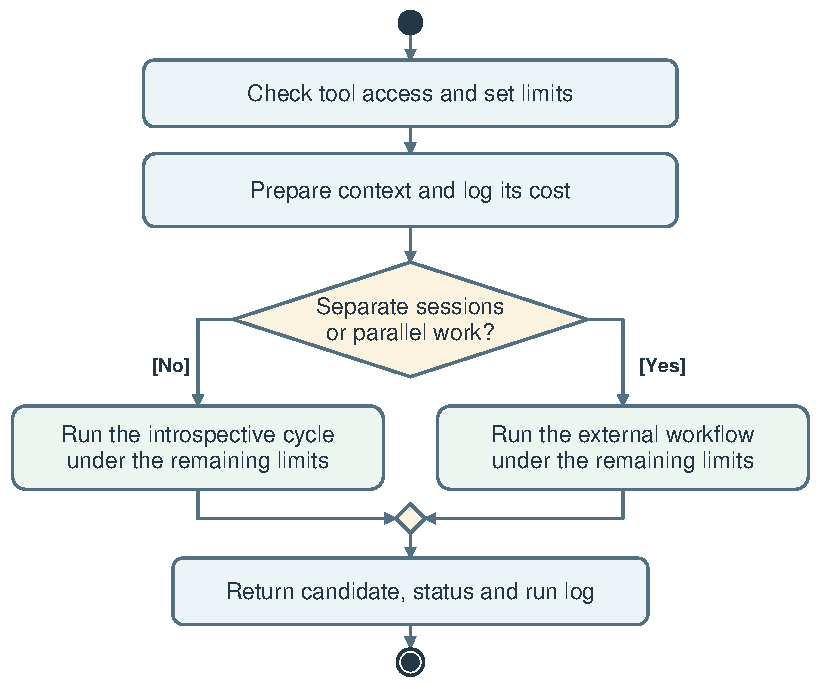
\includegraphics[width=.96\linewidth]{figures/uml-route.pdf}
\caption{Выбор режима и~передача результата. Обе ветви получают оставшиеся лимиты.}\label{fig:uml-route}
\end{figure}
\FloatBarrier
\begin{figure}[!ht]
\centering
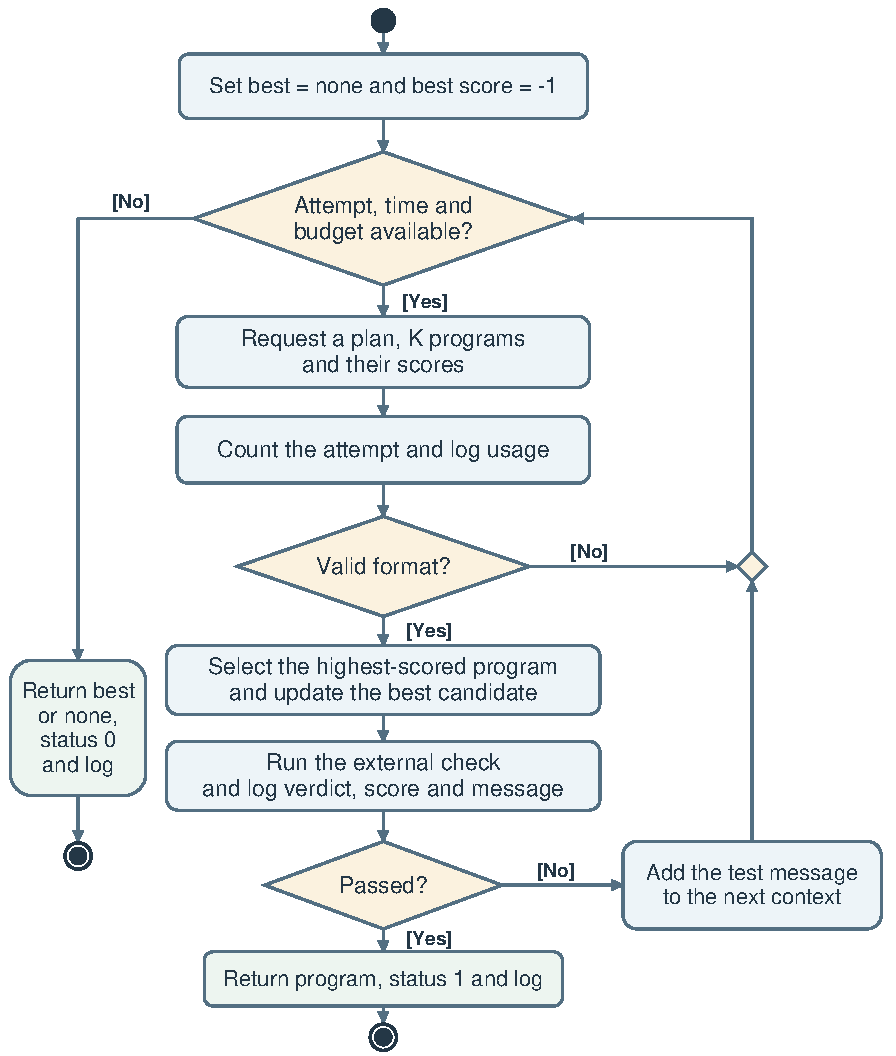
\includegraphics[width=\linewidth,height=.79\textheight,keepaspectratio]{figures/uml-iteration.pdf}
\caption{Интроспективный проход с~проверкой и~ограничением числа попыток. При ошибке формата использованные токены также записываются в~журнал.}\label{fig:uml-iteration}
\end{figure}
\FloatBarrier

\begin{figure}[!ht]
\centering
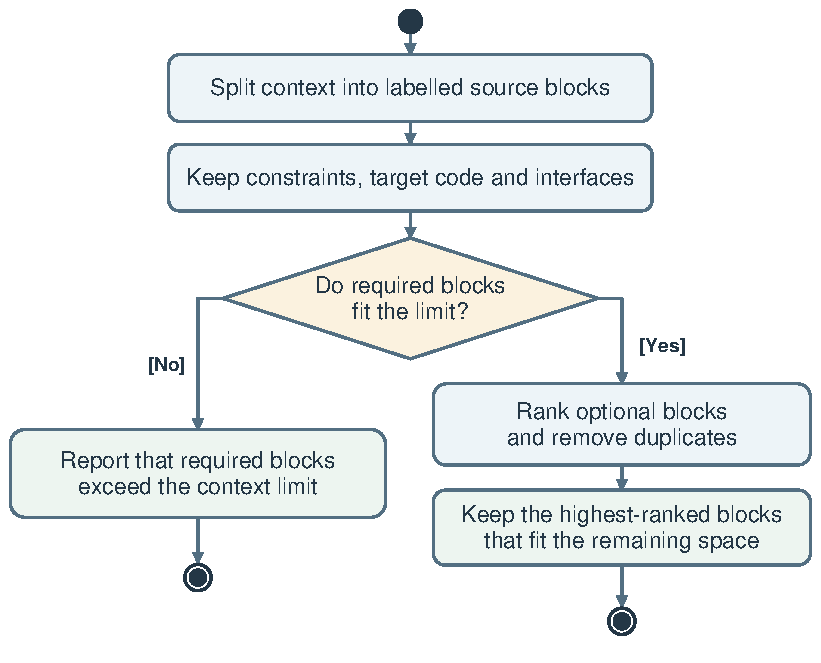
\includegraphics[width=.96\linewidth]{figures/uml-context.pdf}
\caption{Подготовка контекста при включённом сжатии. Если обязательные блоки превышают лимит, контроллер сообщает об~этом до вызова модели.}\label{fig:uml-context}
\end{figure}
\FloatBarrier
\section{Сравнение с~авторской реализацией SCC}\label{subsec:scc}
Self-Collaboration Code Generation, или SCC, сравнивается как более сложная процедура с~взаимодействием ролей и~внутренним исполнением кода. Использован авторский код ревизии \texttt{b471e120}~\cite{scc2024source}. Сохранены классы ролей, инструкции и~логика контроллера. Вызовы адаптированы к~GPT-5.6 Luna через CLI. Число итераций разработчика уменьшено с~четырёх до двух: первоначальный код и~не более одного исправления. Результаты относятся к~этой конфигурации.

Тестировщик SCC создаёт примеры, которые запускаются в~контейнере. Контроллер может остановиться, если выполнение не вызывает исключения. Напечатанные результаты при этом автоматически не сверяются с~ожидаемыми значениями. Поэтому внутреннее завершение SCC ещё не означает успешного решения задачи: окончательная программа отдельно проходит исходные тесты BigCodeBench.

Из 2\,000 назначений каждого метода завершены 1\,600 для SCC, 1\,997 для SR и~1\,998 для SN. Осталось 405 незавершённых запусков: 397 инфраструктурных ошибок и~восемь приостановленных попыток. Большинство ошибок связано с~запуском контейнеров SCC. После контроля среды для SCC доступны 1\,574 оценки, из них 809 успешных. Для SR получено 1\,067 успехов из 1\,964 оценок, для SN --- 1\,064 из 1\,965.

Итоговые тесты и~учёт неуспешных программ остаются такими же, как в~основном сравнении. Однако набор повторов устроен иначе: для задачи заранее выбирались один, два или три повтора, и~часть назначений не завершилась. Поэтому парная оценка SCC использует совпадающие доступные повторы, тогда как в~основной серии требуются все три повтора обоих методов. Сначала разности усредняются внутри задачи, затем задачи получают равные веса. Для SCC минус SR результат равен $-2{,}68$ пункта на 883 задачах с~интервалом $[-4{,}72;-0{,}60]$. Для SCC минус SN получено $-2{,}48$ пункта на 882 задачах с~интервалом $[-4{,}50;-0{,}43]$. Оба значения $p$ после поправки Холма в~отдельном семействе из двух сравнений равны 0,02172.

Большое число пропусков ограничивает этот вывод. Контроль среды прошла 941 из 956 задач этой серии. Если учесть все неизвестные исходы на этих 941 задаче, крайние границы составят $[-12{,}98;+6{,}61]$ пункта относительно SR и~$[-13{,}14;+6{,}43]$ относительно SN. Они допускают оба направления различия. Значит, наблюдаемое преимущество SR и~SN нельзя переносить на всю назначенную выборку SCC.

Для дополнительной проверки сохранены 399 промежуточных программ незавершённых процессов SCC. Из 392 программ на пригодных задачах тесты прошли 196. Это показывает, что инфраструктурный сбой мог прервать процесс уже после появления работающего кода. Но промежуточные программы не подменяют отсутствующий итог контроллера и~не входят в~основную долю успехов SCC.

На полных ресурсных парах отношение средних тарифных оценок SCC/SR равно 3,138 на 896 задачах, а~SCC/SN --- 2,939 на 895. Описательные интервалы составляют $[3{,}07;3{,}21]$ и~$[2{,}87;3{,}01]$. Таким образом, завершённые процедуры SCC с~известными счётчиками требуют больше ресурсов. Неопределённость качества во всей выборке сохраняется из-за пропусков.


\section{Материалы для проверки результатов}\label{app:materials}
Экспериментальная часть сверена с~ревизией \texttt{008b730a} ветки \texttt{FSE-2027} репозитория \href{https://github.com/daniil-novel/article-INoT/tree/008b730a905277079710092ecf3881770eb100fc}{article-INoT}. В~ней доступны архивы ранних серий на 40, 200 и~80 задачах. Данные расширенной серии и~сравнения с~SCC опубликованы в~пакете \path{submission/fse2027/artifact/fse2027-anonymous-analysis-artifact.zip}. Он содержит записи назначений и~сводки: \path{primary/assignment_outcomes.jsonl}, \path{primary/summary.json}, \path{scc/assignment_outcomes.jsonl} и~\path{scc/summary.json}. Этот пакет позволяет пересчитать результаты, но включает не все диалоги и~служебные журналы.

Полные рабочие архивы двух последних серий сохранены локально и~не входят в~указанную ревизию GitHub. Вместе с~ранними сериями они находятся в~следующих папках каталога \path{reproducibility/results}:
\begin{itemize}
\item \path{20260908_codex_mini_dev40}
\item \path{20260908_codex_mini_heldout200}
\item \path{20260908_codex_mini_segregation80}
\item \path{20260912_scale1000_luna_full}
\item \path{20260913_scc2000_luna_full_v2}.
\end{itemize}
Для первых четырёх использованы \path{analysis/summary.json} и~записи отдельных кандидатов. Для SCC использован \path{amended-analysis/summary.json}, который соответствует выбранным 2\,000 сочетаниям «задача--повтор». Он отделён от анализа исходного плана на 9\,000 назначений. Дополнительные анализы сохранены в~материалах \path{submission/fse2027/review}, а~таблицы --- в~\path{submission/fse2027/translation-ru}.

При подготовке этой редакции по сохранённым записям повторно проверены количества запусков, успехи, основные разности и~ресурсные показатели. Для таблицы~\ref{tab:scale-quality-cost} в~архив исходников включён скрипт \path{analysis/quality_and_cost.py}, который принимает файл \path{primary/assignment_outcomes.jsonl} и~пересчитывает показатели на общей выборке. При этом пересчёте использовались архивные ответы GPT-5.6 Luna. Такой пересчёт проверяет согласованность данных и~анализа. Пересчёт использует сохранённые исходы тестов.


Для локального пилота комплект исходников содержит каталог \path{analysis/route-pilot}. В~файле \path{protocol.json} зафиксированы варианты сравнения, ставки для расчёта стоимости и~правило выбора режима. В~\path{tasks.json} перечислены 12 задач и~сетки входных значений. Файл \path{run.py} воспроизводит запросы, порядок запусков и~проверку ответов. До первого измерения в~\path{recorded/manifest.json} сохранены порядок назначений, версия Ollama, идентификатор весов модели и~контрольные суммы протокола, набора задач и~программы запуска.

Каждая запись \path{recorded/runs.jsonl} содержит условие, выбранный режим, все запросы и~ответы, счётчики входа и~выхода, длительность процедуры и~результат проверки. Программа \path{analyze.py} заново проверяет все 60 ответов, сверяет порядок, контрольные суммы и~число вызовов, затем пересчитывает таблицу~\ref{tab:pilot}. Для проверки сохранённых ответов достаточно Python. Для повторной генерации нужна локальная модель Llama~3.2~3B Instruct в~Ollama. Редактируемые исходники диаграмм приложения~\ref{app:uml} находятся в~файле \path{figures/hybrid-activities.drawio}.

\section{Что остаётся за пределами тарифной оценки}\label{app:tco}
Расходы на применение системы включают больше, чем обращения к~модели. Для одного месяца совокупная стоимость владения, или TCO, записывается как
\begin{formulakey}
\begin{equation}
\mathrm{TCO}_{\mathrm{month}}=
C_{\mathrm{inf,month}}+C_{\mathrm{hw}}+C_{\mathrm{energy}}+
C_{\mathrm{storage}}+C_{\mathrm{ops}}.
\end{equation}
\begin{symbols}
\sym{\mathrm{TCO}_{\mathrm{month}}}{совокупная стоимость эксплуатации за месяц}
\sym{C_{\mathrm{inf,month}}}{платежи за обращения к~моделям в~этом месяце}
\sym{C_{\mathrm{hw}},\,C_{\mathrm{energy}}}{аренда или амортизация оборудования и~затраты на электроэнергию}
\sym{C_{\mathrm{storage}},\,C_{\mathrm{ops}}}{хранение данных и~сопровождение, включая труд специалистов}
\end{symbols}
\end{formulakey}
Все слагаемые выражены в~одной валюте за один период. Расход, уже включённый в~тариф сервиса, учитывается один раз.

В~сериях BigCodeBench измерены счётчики токенов и~рассчитана их тарифная стоимость. Полная стоимость внедрения не измерялась. Например, сложная проверка кода может потребовать дополнительных серверов и~ручного разбора ошибок. Поэтому отношение 2,78 из основного эксперимента характеризует только расчётные затраты на модель, а~не расходы организации в~целом.

\end{document}
